% Options for packages loaded elsewhere
\PassOptionsToPackage{unicode}{hyperref}
\PassOptionsToPackage{hyphens}{url}
%
\documentclass[
  ignorenonframetext,
]{beamer}
\usepackage{pgfpages}
\setbeamertemplate{caption}[numbered]
\setbeamertemplate{caption label separator}{: }
\setbeamercolor{caption name}{fg=normal text.fg}
\beamertemplatenavigationsymbolsempty
% Prevent slide breaks in the middle of a paragraph
\widowpenalties 1 10000
\raggedbottom
\setbeamertemplate{part page}{
  \centering
  \begin{beamercolorbox}[sep=16pt,center]{part title}
    \usebeamerfont{part title}\insertpart\par
  \end{beamercolorbox}
}
\setbeamertemplate{section page}{
  \centering
  \begin{beamercolorbox}[sep=12pt,center]{part title}
    \usebeamerfont{section title}\insertsection\par
  \end{beamercolorbox}
}
\setbeamertemplate{subsection page}{
  \centering
  \begin{beamercolorbox}[sep=8pt,center]{part title}
    \usebeamerfont{subsection title}\insertsubsection\par
  \end{beamercolorbox}
}
\AtBeginPart{
  \frame{\partpage}
}
\AtBeginSection{
  \ifbibliography
  \else
    \frame{\sectionpage}
  \fi
}
\AtBeginSubsection{
  \frame{\subsectionpage}
}
\usepackage{amsmath,amssymb}
\usepackage{lmodern}
\usepackage{iftex}
\ifPDFTeX
  \usepackage[T1]{fontenc}
  \usepackage[utf8]{inputenc}
  \usepackage{textcomp} % provide euro and other symbols
\else % if luatex or xetex
  \usepackage{unicode-math}
  \defaultfontfeatures{Scale=MatchLowercase}
  \defaultfontfeatures[\rmfamily]{Ligatures=TeX,Scale=1}
\fi
% Use upquote if available, for straight quotes in verbatim environments
\IfFileExists{upquote.sty}{\usepackage{upquote}}{}
\IfFileExists{microtype.sty}{% use microtype if available
  \usepackage[]{microtype}
  \UseMicrotypeSet[protrusion]{basicmath} % disable protrusion for tt fonts
}{}
\makeatletter
\@ifundefined{KOMAClassName}{% if non-KOMA class
  \IfFileExists{parskip.sty}{%
    \usepackage{parskip}
  }{% else
    \setlength{\parindent}{0pt}
    \setlength{\parskip}{6pt plus 2pt minus 1pt}}
}{% if KOMA class
  \KOMAoptions{parskip=half}}
\makeatother
\usepackage{xcolor}
\newif\ifbibliography
\usepackage{longtable,booktabs,array}
\usepackage{calc} % for calculating minipage widths
\usepackage{caption}
% Make caption package work with longtable
\makeatletter
\def\fnum@table{\tablename~\thetable}
\makeatother
\usepackage{graphicx}
\makeatletter
\def\maxwidth{\ifdim\Gin@nat@width>\linewidth\linewidth\else\Gin@nat@width\fi}
\def\maxheight{\ifdim\Gin@nat@height>\textheight\textheight\else\Gin@nat@height\fi}
\makeatother
% Scale images if necessary, so that they will not overflow the page
% margins by default, and it is still possible to overwrite the defaults
% using explicit options in \includegraphics[width, height, ...]{}
\setkeys{Gin}{width=\maxwidth,height=\maxheight,keepaspectratio}
% Set default figure placement to htbp
\makeatletter
\def\fps@figure{htbp}
\makeatother
\setlength{\emergencystretch}{3em} % prevent overfull lines
\providecommand{\tightlist}{%
  \setlength{\itemsep}{0pt}\setlength{\parskip}{0pt}}
\setcounter{secnumdepth}{-\maxdimen} % remove section numbering
\ifLuaTeX
  \usepackage{selnolig}  % disable illegal ligatures
\fi
\IfFileExists{bookmark.sty}{\usepackage{bookmark}}{\usepackage{hyperref}}
\IfFileExists{xurl.sty}{\usepackage{xurl}}{} % add URL line breaks if available
\urlstyle{same} % disable monospaced font for URLs
\hypersetup{
  pdftitle={Metagenomic Barcoding},
  pdfauthor={Reed Clark Benkendorf Northwestern University \& The Chicago Botanic Garden Southwest Conservation Corps \& Bureau of the Land Management},
  hidelinks,
  pdfcreator={LaTeX via pandoc}}

\title{Metagenomic Barcoding}
\subtitle{of Pollen Loads Offers Insights onthe Foraging Patterns of
Queen Bumble Bees}
\author{Reed Clark BenkendorfNorthwestern University \& The Chicago
Botanic GardenSouthwest Conservation Corps \& Bureau of the Land
Management}
\date{March 1\textsuperscript{st}, '23}

\begin{document}
\frame{\titlepage}

\begin{frame}
\end{frame}

\begin{frame}{Overview}
\protect\hypertarget{overview}{}
1 \textbar{} background

2 \textbar{} questions

3 \textbar{} approaches

4 \textbar{} methods

5 \textbar{} results

6 \textbar{} future

7 \textbar{} conclusions

\begin{figure}
\centering
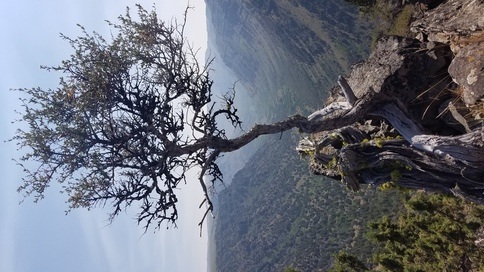
\includegraphics{../graphics/pictures/Cercocarpus-Steens.resized.jpg}
\caption{ \emph{Cercocarpus} }
\end{figure}
\end{frame}

\begin{frame}{Team}
\protect\hypertarget{team}{}
Jane Ogilvie \emph{(ecological fieldwork, design)}

Emily J. Woodworth \emph{(pollen morphology, and microscopy)}

Sophie Taddeo \emph{(geo-spatial, statistics)}

Paul CaraDonna \emph{(little bees/big picture(s))}

Jeremie Fant \emph{(all things molecular and tied together)}

\emph{i.e.} an in-house production.
\end{frame}

\begin{frame}{the world is big - 1.1}
\protect\hypertarget{the-world-is-big---1.1}{}
\begin{figure}
\centering
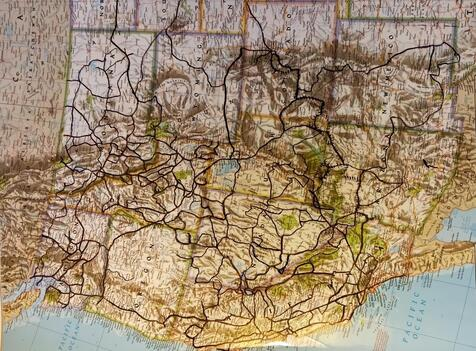
\includegraphics{../graphics/pictures/major_roads.resized.jpg}
\caption{Primary Roads}
\end{figure}
\end{frame}

\begin{frame}{\ldots{} \emph{really really} big - 1.2}
\protect\hypertarget{really-really-big---1.2}{}
\begin{itemize}
\tightlist
\item
  5 sampling seasons (May - October)
\item
  3 person crews
\item
  2 partial support personnel
\item
  281 plots
\item
  area of inference: \textasciitilde{} 900,000 acres
\item
  0.363\% of Bureau of Land Management administered land
\end{itemize}

\begin{figure}
\centering
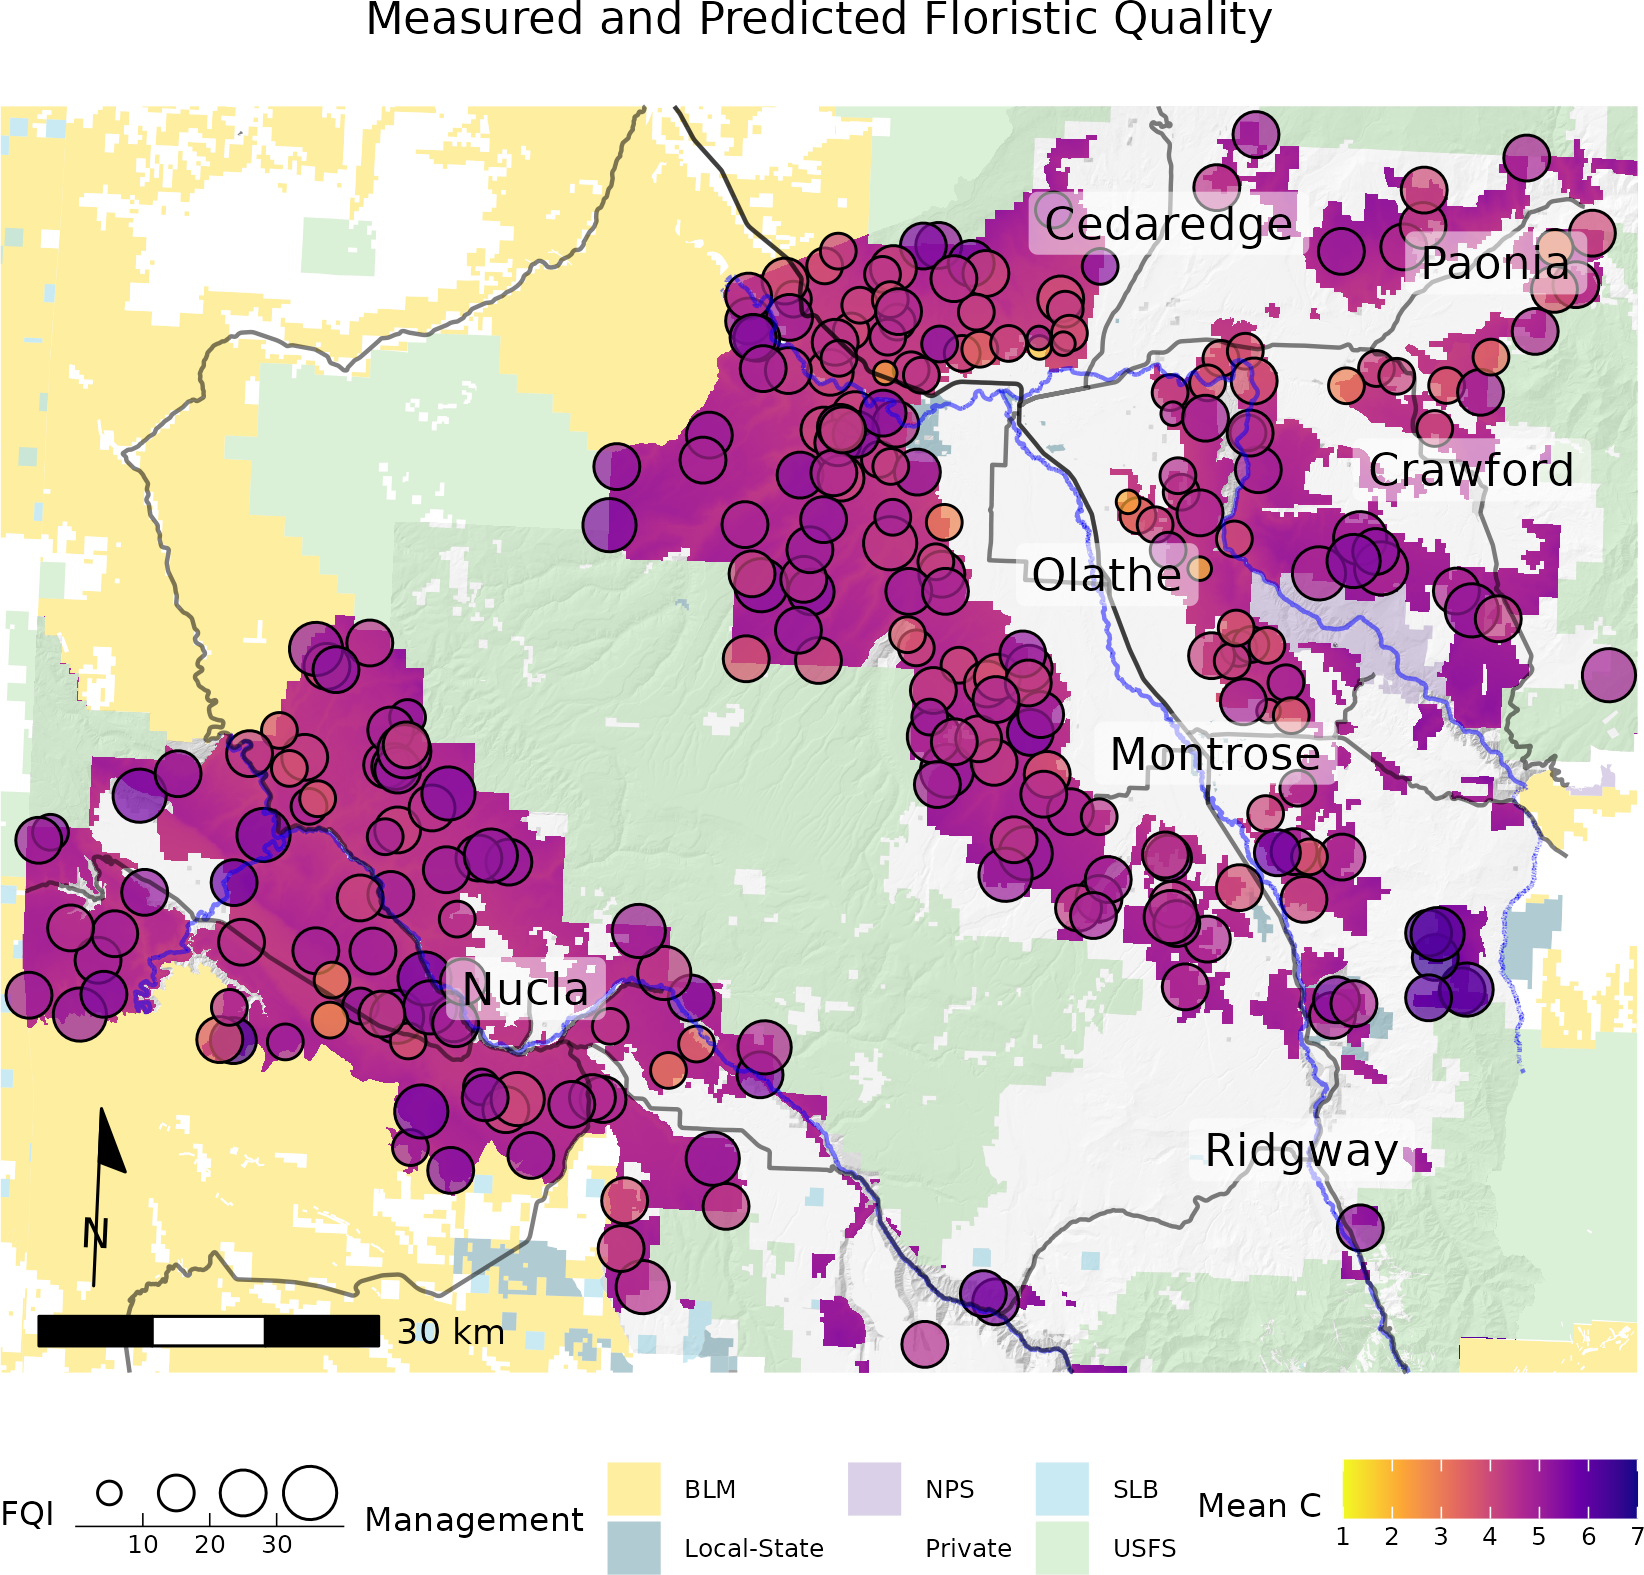
\includegraphics[width=0.85\textwidth,height=\textheight]{../graphics/assorted/FQI.png}
\caption{FQI calculated from AIM}
\end{figure}
\end{frame}

\begin{frame}{funding opportunties - 1.3}
\protect\hypertarget{funding-opportunties---1.3}{}

\includegraphics{../graphics/pictures/Nelson.jpg} \#\# how do we sample
the planet? - 1.4
\end{frame}

\begin{frame}{plant species in ecology - 1.6}
\protect\hypertarget{plant-species-in-ecology---1.6}{}
\begin{itemize}
\tightlist
\item
  mis-identification is \emph{very} common
\item
  mis-identification can lead to nebulous understandings
\item
  mis-identification can lead to mis-management
\end{itemize}

\begin{figure}
\centering
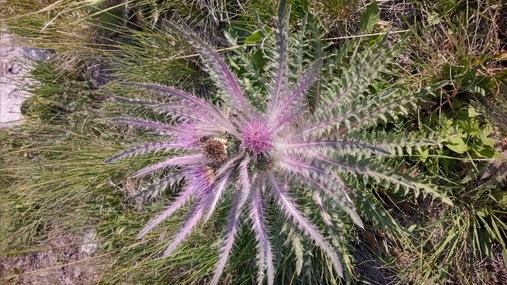
\includegraphics{../graphics/pictures/Cirsium_scariosum.resized.jpg}
\caption{\emph{Cirsium scariosum}}
\end{figure}
\end{frame}

\begin{frame}{insects species in ecology - 1.7}
\protect\hypertarget{insects-species-in-ecology---1.7}{}
\begin{itemize}
\tightlist
\item
  Macro Invertebrates

  \begin{itemize}
  \tightlist
  \item
    stream ecology bio indicators

    \begin{itemize}
    \tightlist
    \item
      mayflies, caddisflies, stoneflies\\
    \end{itemize}
  \end{itemize}
\item
  Coleoptera

  \begin{itemize}
  \tightlist
  \item
    soil contamination by metal
  \end{itemize}
\item
  \emph{from bio-indicators to foci?}
\end{itemize}

\begin{figure}
\centering
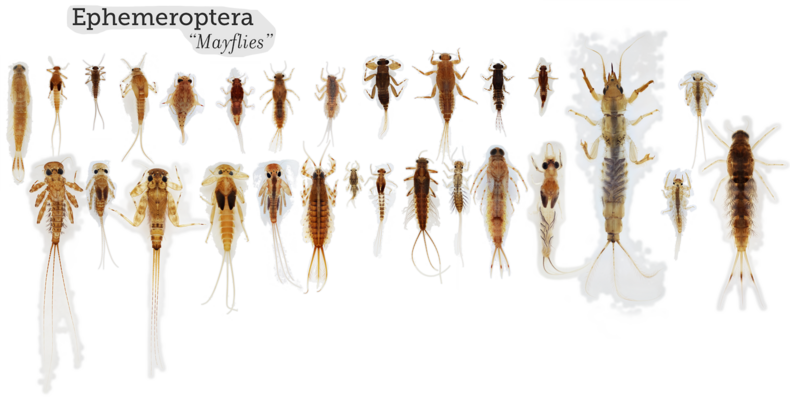
\includegraphics[width=0.5\textwidth,height=\textheight]{../graphics/assorted/ephemeroptera.resized.png}
\caption{\emph{Macroinvertebrates.org}}
\end{figure}
\end{frame}

\begin{frame}{from organisms to interactions - 1.8}
\protect\hypertarget{from-organisms-to-interactions---1.8}{}
\begin{itemize}
\tightlist
\item
\item
  Bullet 2
\item
  Bullet 3
\end{itemize}

\begin{figure}
\centering
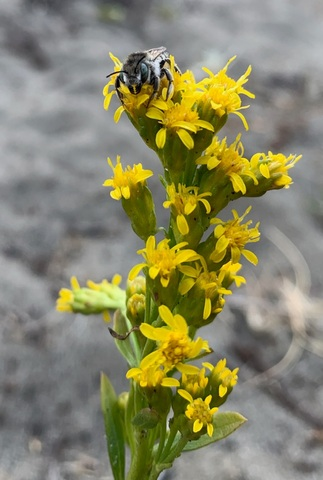
\includegraphics[width=0.85\textwidth,height=\textheight]{../graphics/pictures/Megachile_Solidago.resized.jpg}
\caption{\emph{Solidago spathulata} \& \emph{Megachile wheeleri}, by A.
Litz}
\end{figure}
\end{frame}

\begin{frame}{metabarcoding - 1.10}
\protect\hypertarget{metabarcoding---1.10}{}
\begin{itemize}
\tightlist
\item
  Barcoding

  \begin{itemize}
  \tightlist
  \item
    molecular identification of tissue from a single organism
  \end{itemize}
\item
  Metabarcoding

  \begin{itemize}
  \tightlist
  \item
    molecular identification of organisms present in a mixed substrate
  \end{itemize}
\end{itemize}

\begin{figure}
\centering
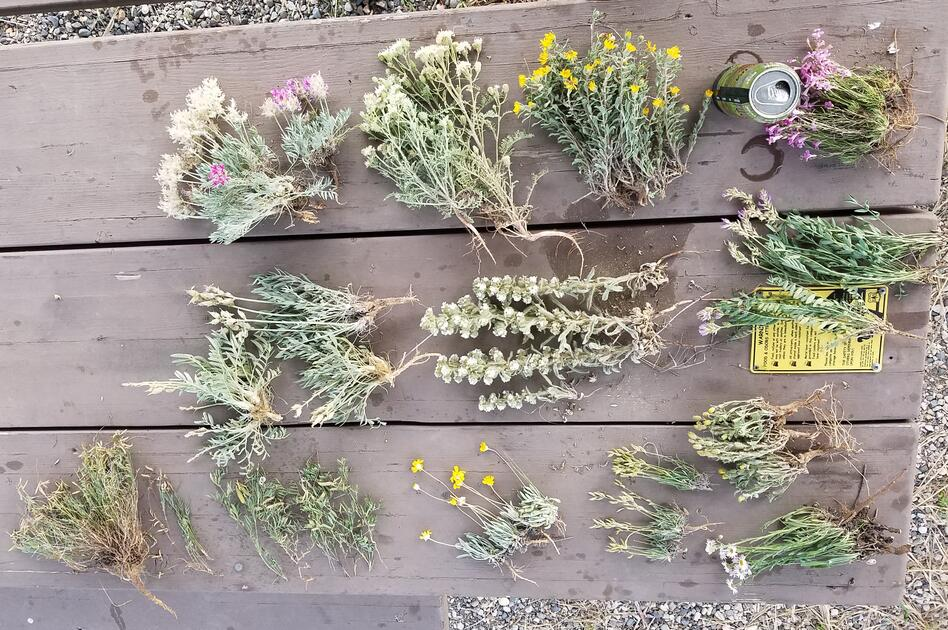
\includegraphics[width=0.8\textwidth,height=\textheight]{../graphics/pictures/Five_Astragali.jpg}
\caption{Five Astragali}
\end{figure}

\note{Quick definition check, so barcoding is simply the identification
of tissue from one organism, e.g.~we could try and identify the species
of Astragalus from this day of collecting via barcoding; assuming they
were present in a database. `Meta' just means we have a pooled sample to
deal with, these are generally samples of soil, pollen, or water. So if
we wanted to identify the assembly of organisms which are present on the
rhizosphere of a species of Astragalus, we would use metabarcoding.}
\end{frame}

\begin{frame}{barcodes - 1.11}
\protect\hypertarget{barcodes---1.11}{}
\begin{itemize}
\tightlist
\item
  Kingdom: Animal,

  \begin{itemize}
  \tightlist
  \item
    COI (\textbf{C}ytochrome c \textbf{O}x\textbf{I}dase)
  \item
    \emph{holding it's own in Fungi}
  \end{itemize}
\item
  Kingdoms: Fungi + Plant

  \begin{itemize}
  \tightlist
  \item
    ITS (\textbf{I}nteral \textbf{T}ranscribed \textbf{S}pacer)
  \item
    \emph{holding it's own in Fungi}
  \end{itemize}
\item
  Kingdom: Plant

  \begin{itemize}
  \tightlist
  \item
    ITS, rbcL, matK, trnH-psbA
  \item
    \emph{\textbf{not} holding much of anything}
  \end{itemize}
\end{itemize}
\end{frame}

\begin{frame}{new barcodes for plants? - 1.12}
\protect\hypertarget{new-barcodes-for-plants---1.12}{}
\begin{itemize}
\tightlist
\item
  genomics

  \begin{itemize}
  \tightlist
  \item
    low cost
  \item
    high coverage
  \item
    PCR free?
  \end{itemize}
\item
  reference library ?

  \begin{itemize}
  \tightlist
  \item
    old barcode library in development for nearly 20 years
  \item
    Kew PAFTOL
  \end{itemize}
\item
  angiosperms 353
\end{itemize}

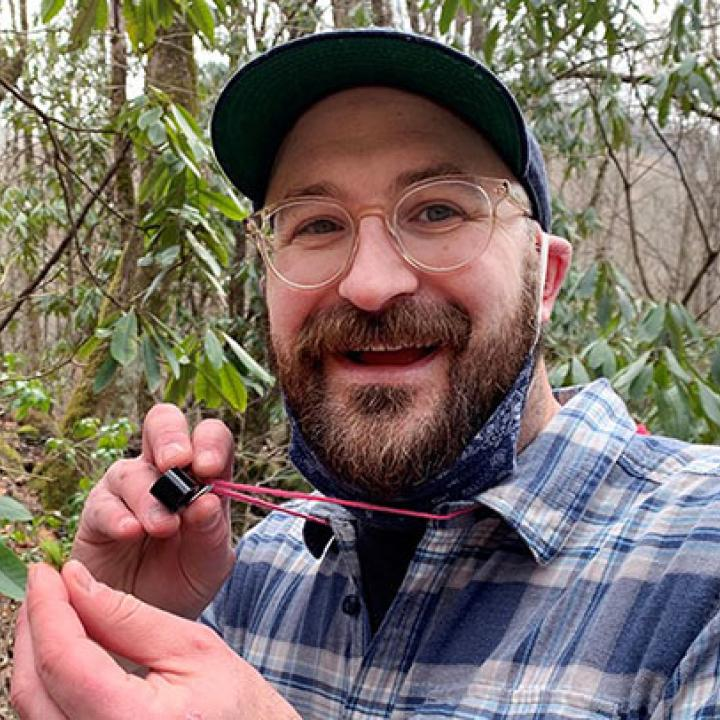
\includegraphics[width=0.5\textwidth,height=\textheight]{../graphics/pictures/norm-wickett.jpg}

\includegraphics[width=0.4\textwidth,height=\textheight]{../graphics/pictures/matt-johnson.jpg}
\end{frame}

\begin{frame}{2 - questions}
\protect\hypertarget{questions}{}
\end{frame}

\begin{frame}{scale - from plots to continents?}
\protect\hypertarget{scale---from-plots-to-continents}{}
\begin{itemize}
\tightlist
\item
  many questions will be approached using two perspectives

  \begin{itemize}
  \tightlist
  \item
    bottom up i.e.~plot based data collected by Jane
  \item
    top down i.e.~computer based data generated by me
  \end{itemize}
\item
  fine scale data serving to as ground truth to the computer generated
  models
\end{itemize}
\end{frame}

\begin{frame}{can we predict what is flowering in time \& space? - 2.1}
\protect\hypertarget{can-we-predict-what-is-flowering-in-time-space---2.1}{}
\begin{itemize}
\tightlist
\item
  \textbf{which species are present in an area?}
\item
  \textbf{when are these species flowering in an area?}
\item
  diverse clades provide challenges for identification
\item
  species often diverged in ecological traits
\end{itemize}

\begin{figure}
\centering
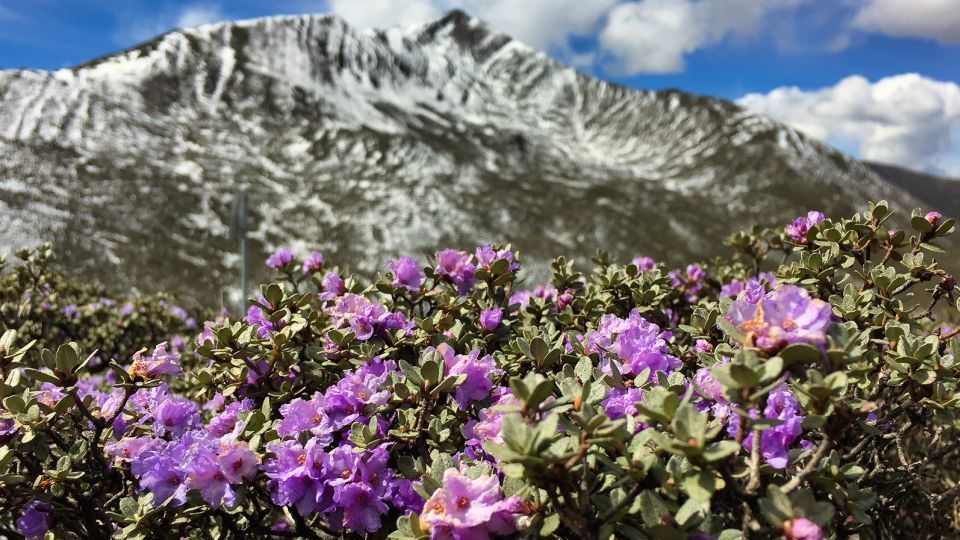
\includegraphics[width=0.45\textwidth,height=\textheight]{../graphics/pictures/Rhododendron_QinLi.jpg}
\caption{\emph{Rhododendron} sp. Hengduan Mtns., by Qin Li}
\end{figure}
\end{frame}

\begin{frame}{do a353 work as barcodes? - 2.2}
\protect\hypertarget{do-a353-work-as-barcodes---2.2}{}
\begin{itemize}
\tightlist
\item
  `universal' markers for phylogenomics
\item
  usable in all flowering plant clades
\item
  first comprehensive genus level phylogeny of flowering plants
\item
  shoot the moon; meta genomics first
\end{itemize}

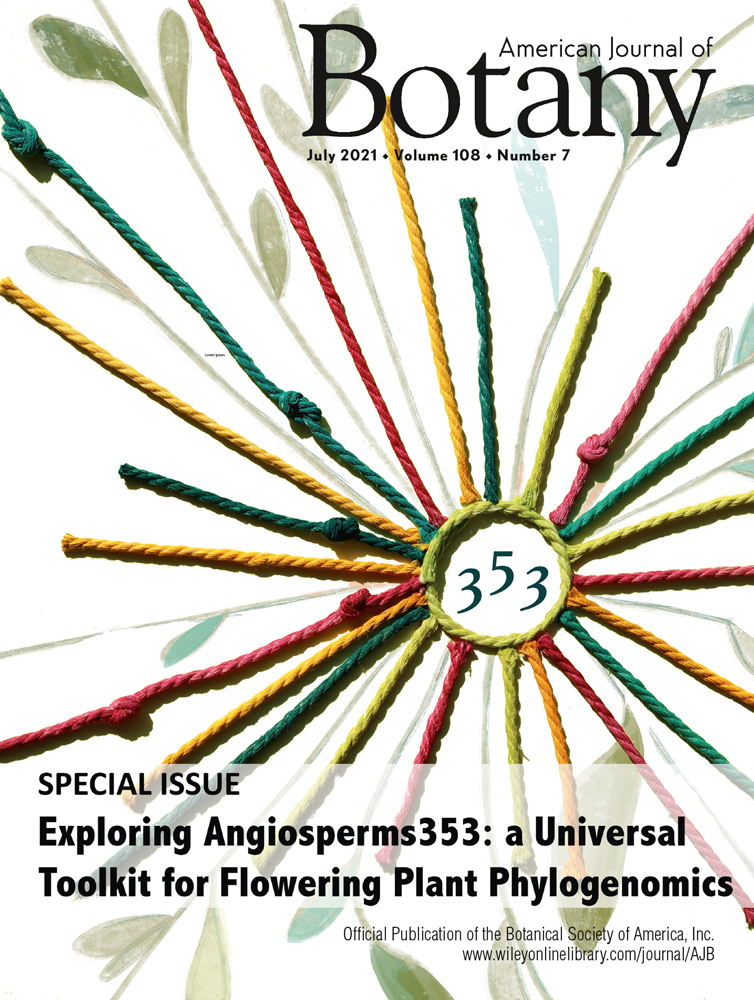
\includegraphics[width=0.9\textwidth,height=\textheight]{../graphics/pictures/Angiosperms353.jpg}
\end{frame}

\begin{frame}{are a353 semi-quantitative? - 2.3}
\protect\hypertarget{are-a353-semi-quantitative---2.3}{}
Do the number of sequence reads reflect the amount of biological
material in a sample?
\end{frame}

\begin{frame}{3 - approaches}
\protect\hypertarget{approaches}{}
\end{frame}

\begin{frame}{predict what is flowering; \emph{Time \& Space} - 3.1}
\protect\hypertarget{predict-what-is-flowering-time-space---3.1}{}
\begin{itemize}
\tightlist
\item
  no longer any funding for floristics; few Floras maintained, fewer
  written
\item
  essentially no funding remains for alpha taxonomy
\item
  little to no funding natural history
\item
  how do we monitor ecological shifts under climate change?

  \begin{itemize}
  \tightlist
  \item
    geographic ranges
  \item
    flowering time
  \end{itemize}
\item
  \textbf{\emph{back to the sheets!}}
\end{itemize}

\begin{figure}
\centering
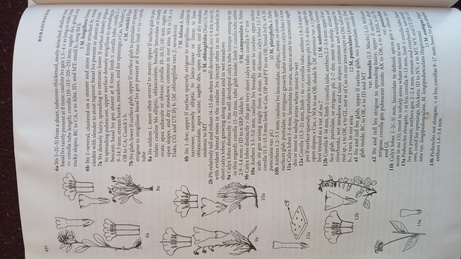
\includegraphics[width=\textwidth,height=0.8\textheight]{../graphics/pictures/fpnw2.resized.jpg}
\caption{FPNW 2\textsuperscript{nd}}
\end{figure}
\end{frame}

\begin{frame}{custom sequence databases; \emph{a353 as barcodes?} - 3.2}
\protect\hypertarget{custom-sequence-databases-a353-as-barcodes---3.2}{}
\begin{itemize}
\tightlist
\item
  reduce number of species present in database

  \begin{itemize}
  \tightlist
  \item
    reduce computational requirements
  \item
    increase likelihood of relevant matches across loci
  \item
    reduce false positives for semi-quantitative inference
  \end{itemize}
\end{itemize}
\end{frame}

\begin{frame}{queen bee pollen loads: \emph{a353 as barcodes?} - 3.3}
\protect\hypertarget{queen-bee-pollen-loads-a353-as-barcodes---3.3}{}
\begin{itemize}
\item
  DNA extracted from corbiculae loads

  \begin{itemize}
  \tightlist
  \item
    a `pollen basket' for holding grains collected grains
  \end{itemize}
\item
  variable in size, but generally many tens of thousands of grains

  \begin{figure}
  \centering
  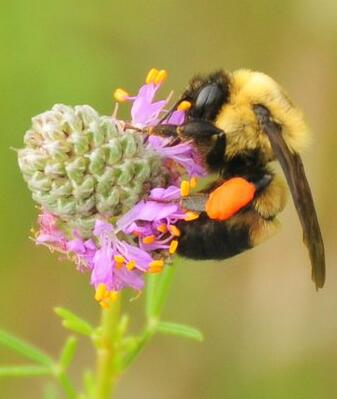
\includegraphics{../graphics/pictures/Corbiculae-FWS.jpeg}
  \caption{USFWS}
  \end{figure}
\end{itemize}
\end{frame}

\begin{frame}{identify pollen grains; \emph{a353 semi-quantitative?} -
3.4}
\protect\hypertarget{identify-pollen-grains-a353-semi-quantitative---3.4}{}
\begin{itemize}
\tightlist
\item
\end{itemize}
\end{frame}

\begin{frame}{4 - methods}
\protect\hypertarget{methods}{}
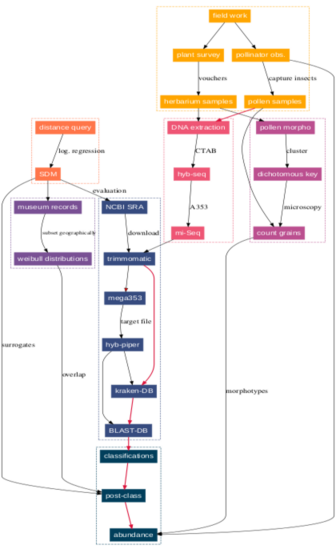
\includegraphics{../graphics/plots/flowchart.resized.png}

\begin{itemize}
\tightlist
\item
  field work
\item
  spatial
\item
  temporal\\
\item
  morphologic\\
\item
  laboratory\\
\item
  bioinformatic\\
\item
  post-classification\\
\end{itemize}
\end{frame}

\begin{frame}{study system \& field work - 4.1}
\protect\hypertarget{study-system-field-work---4.1}{}
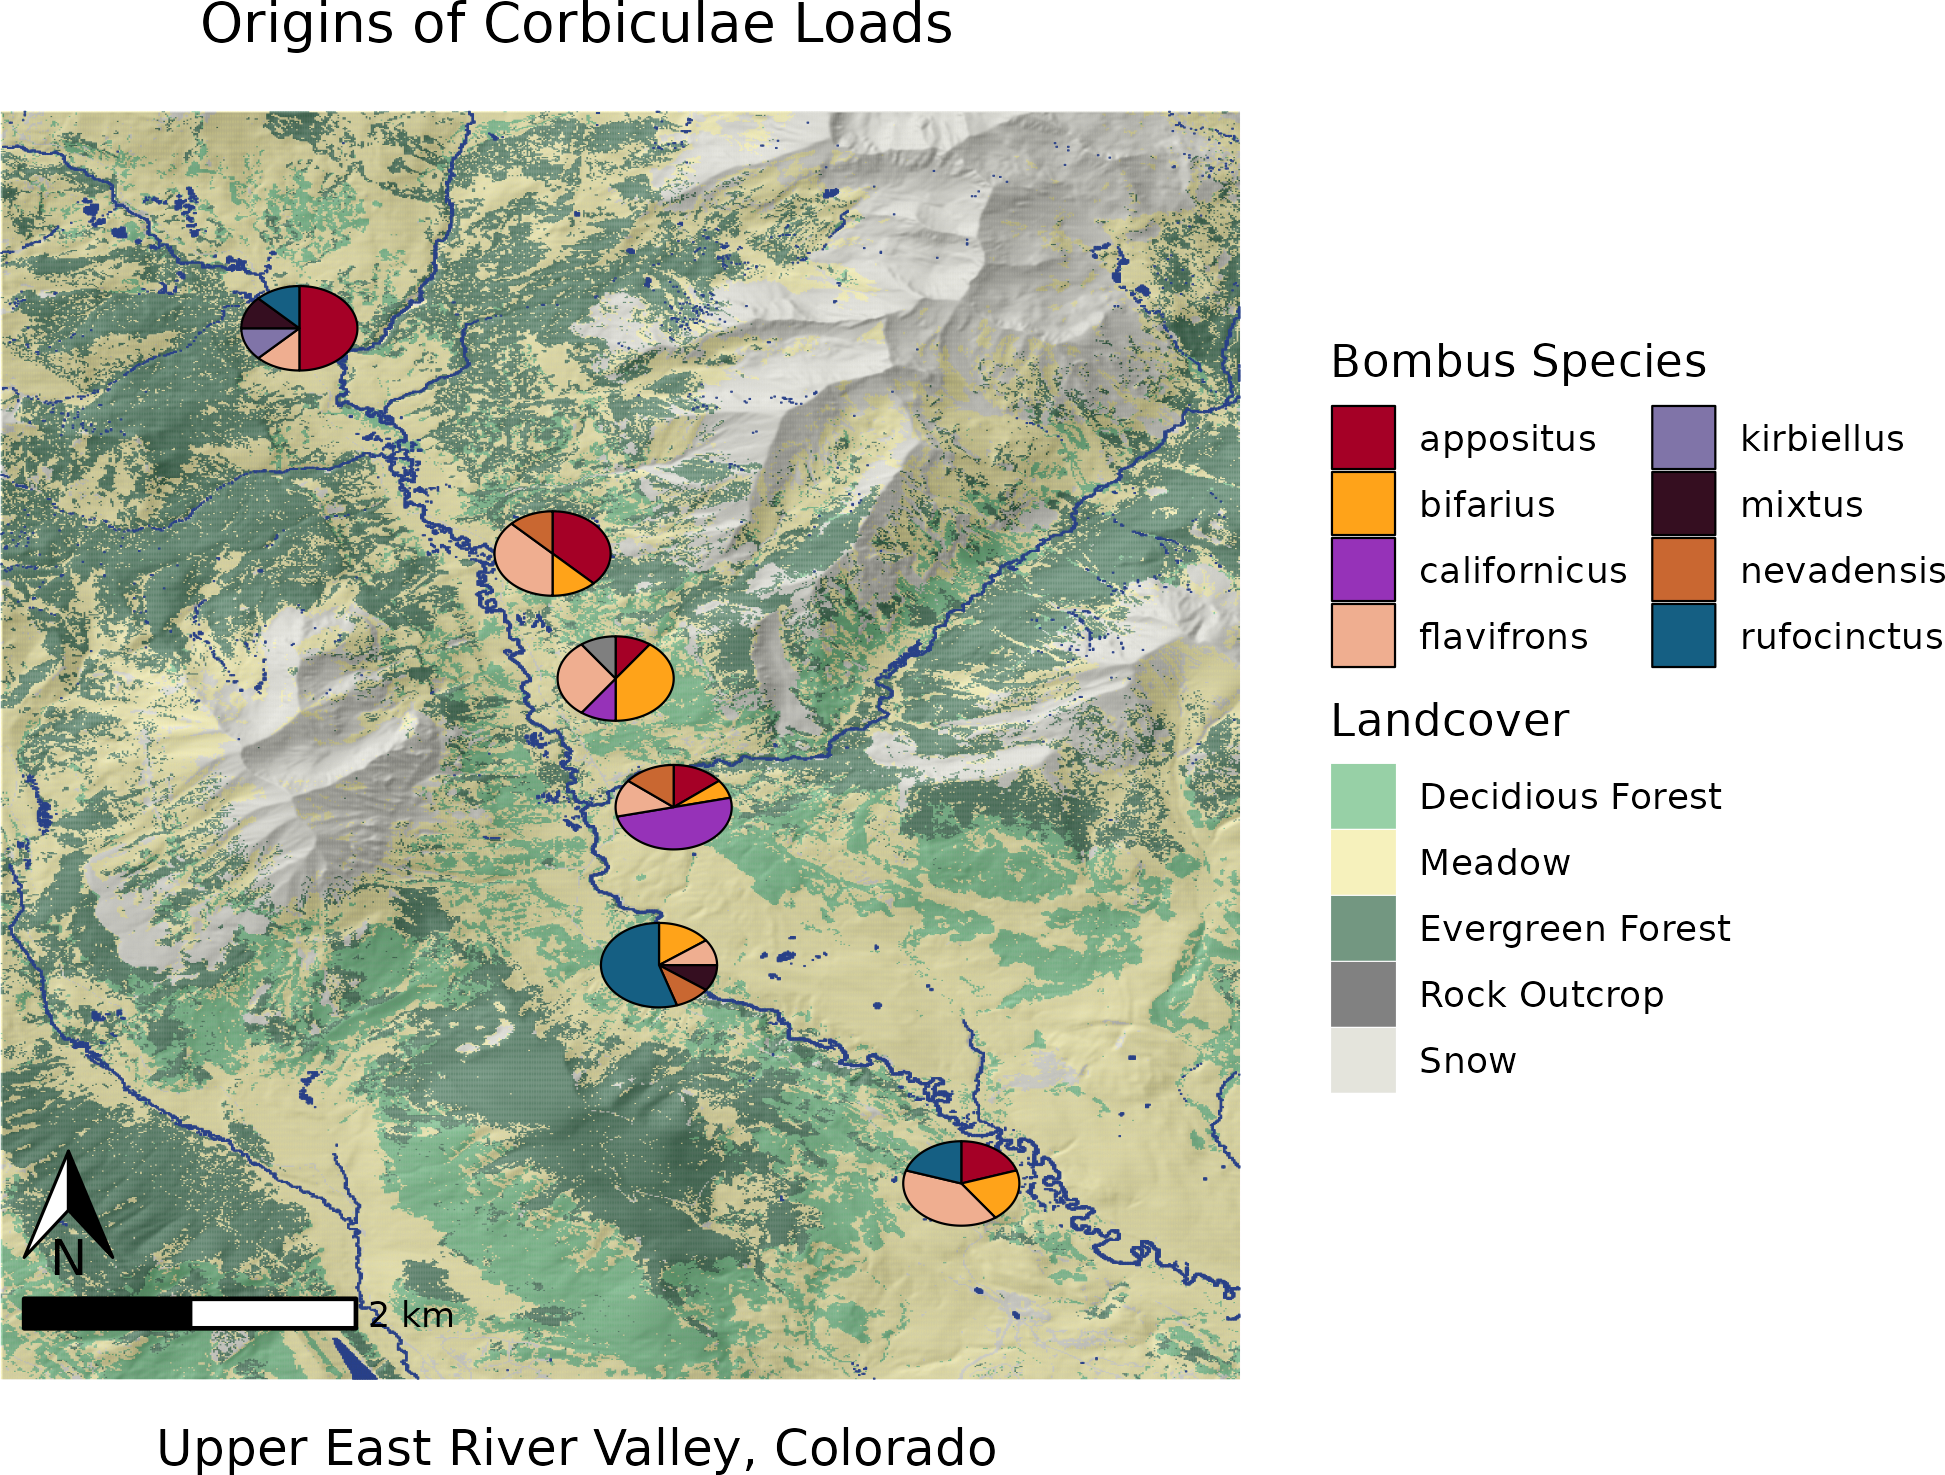
\includegraphics[width=0.7\textwidth,height=\textheight]{../graphics/plots/siteMaps.png}
\end{frame}

\begin{frame}{pollen morphological identification 4.2}
\protect\hypertarget{pollen-morphological-identification-4.2}{}
\begin{itemize}
\tightlist
\item
  Develop grain reference library
\item
  Score traits
\item
  write keys
\item
  Emily Woodworth talk at
  \href{https://2021.botanyconference.org/engine/search/index.php?func=detail\&aid=924}{`Not
  Another Specimen'} ASPT @ Botany 2021
\end{itemize}

\begin{figure}
\centering
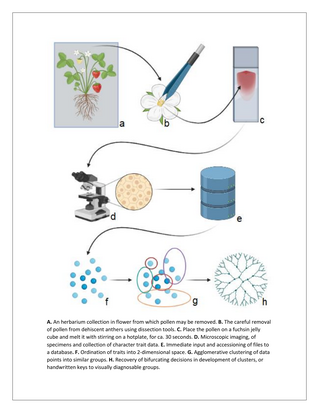
\includegraphics[width=0.93\textwidth,height=\textheight]{../graphics/assorted/mircoscopy_workflow.resized.png}
\caption{workflow}
\end{figure}
\end{frame}

\begin{frame}{pollen reference library 4.2.1}
\protect\hypertarget{pollen-reference-library-4.2.1}{}
\begin{itemize}
\tightlist
\item
  ca. 110 species
\item
  60 novels species added
\item
  ca. 1/3 of species with duplicate preparations
\item
  shared
\item
  \emph{many more species to add to key!! (60 +, mostly un- sampled
  families)}
\end{itemize}

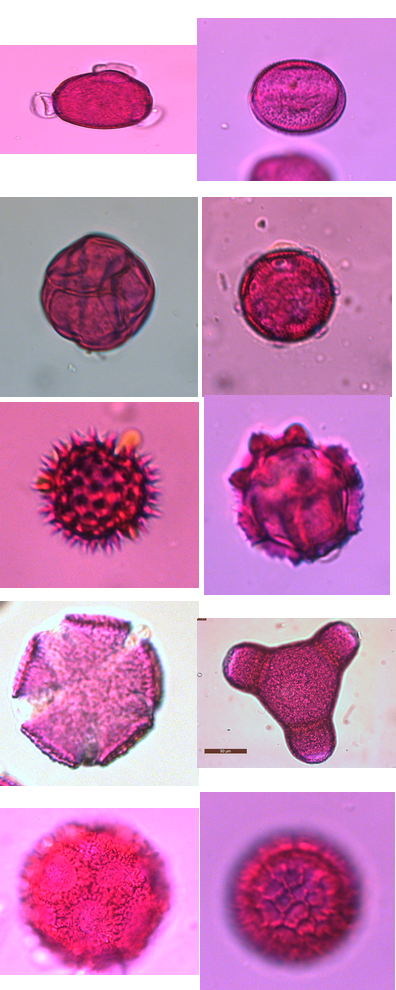
\includegraphics[width=0.65\textwidth,height=\textheight]{../graphics/pictures/pollen_montage.png}
\end{frame}

\begin{frame}{pollen corbiculae loads 4.2.2}
\protect\hypertarget{pollen-corbiculae-loads-4.2.2}{}
\begin{itemize}
\tightlist
\item
  aliquot from same sample used for molecular\\
\item
  stained by fuchsin jelly with stirring
\item
  transects\\
\item
  rarefaction curves

  \begin{itemize}
  \tightlist
  \item
    richness\\
  \item
    abundance
  \end{itemize}
\end{itemize}

\begin{figure}
\centering
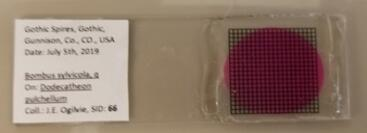
\includegraphics[width=0.3\textwidth,height=\textheight]{../graphics/pictures/corbiculae_slide.resized.jpg}
\caption{Corbiculae Sample}
\end{figure}
\end{frame}

\begin{frame}{molecular barcoding 4.3}
\protect\hypertarget{molecular-barcoding-4.3}{}
\begin{itemize}
\tightlist
\item
  Angiosperms 353\ldots{}
\end{itemize}
\end{frame}

\begin{frame}{spatial analysis 4.3.1}
\protect\hypertarget{spatial-analysis-4.3.1}{}
\begin{itemize}
\tightlist
\item
  2-stage approach

  \begin{itemize}
  \tightlist
  \item
    1\textsuperscript{st}: distance search of records from museums \&
    plot based data (e.g.~Forest Servce)
  \item
    2\textsuperscript{nd}: species distribution modelling
  \end{itemize}
\end{itemize}
\end{frame}

\begin{frame}{plant species, distribution modelling 4.3.1.1.}
\protect\hypertarget{plant-species-distribution-modelling-4.3.1.1.}{}
\begin{itemize}
\tightlist
\item
  develop a candidate species list for barcoding\\
\item
  download all herbarium records from a distance exceeding the study
  area
\item
  compare to known species at field site
\item
  logistic regression
\item
  bootstrapped samples of records
\end{itemize}

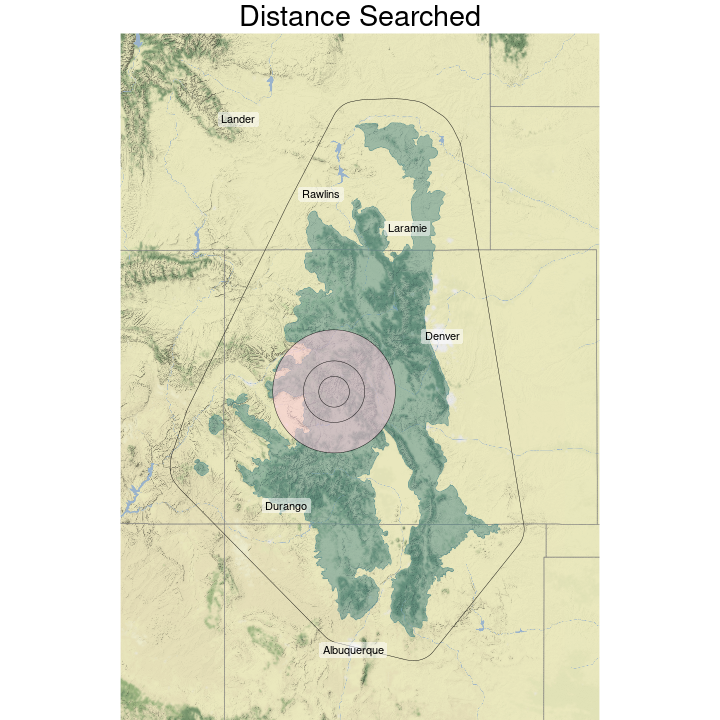
\includegraphics[width=1.05\textwidth,height=\textheight]{../graphics/plots/distance_queried.png}

\note{}
\end{frame}

\begin{frame}{species distribution modelling - 4.3.1.2}
\protect\hypertarget{species-distribution-modelling---4.3.1.2}{}
\begin{itemize}
\tightlist
\item
  gather records from aggregator websites - BIEN
\item
  prune records and model
\item
  GLM \& GAM, RF \& boosting
\item
  ensemble individual models
\item
  \href{https://github.com/sagesteppe/Analytical_Toolkit_SDM}{talk for
  analytical toolkit (PBC 470)}
\end{itemize}

\begin{figure}
\centering
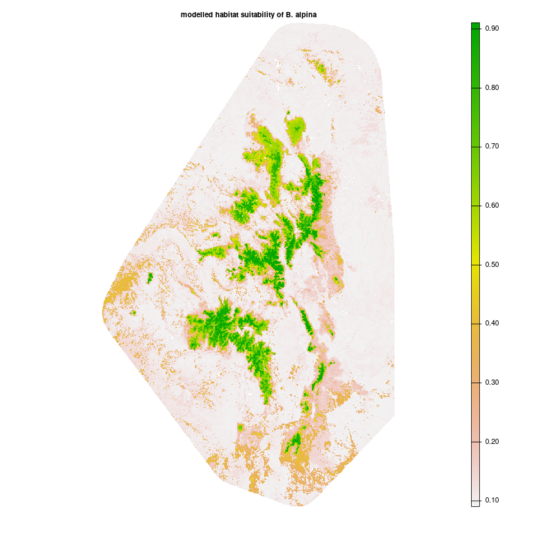
\includegraphics{../graphics/plots/besseya_predicted.resized.png}
\caption{a single species}
\end{figure}
\end{frame}

\begin{frame}{sdm evaluations - 4.3.1.2}
\protect\hypertarget{sdm-evaluations---4.3.1.2}{}
\begin{itemize}
\tightlist
\item
  in pipeline, True skill statistics

  \begin{itemize}
  \tightlist
  \item
    works well over wide range of occurrence records
  \end{itemize}
\end{itemize}
\end{frame}

\begin{frame}{temporal modelling - 4.3.2}
\protect\hypertarget{temporal-modelling---4.3.2}{}
\begin{itemize}
\tightlist
\item
  reduce herbarium records to study domain
\item
  thin records to analogous ecoregions
\item
  trim start/end records
\item
  identify major phenological cues, subset records to similar areas
\end{itemize}
\end{frame}

\begin{frame}{temporal modelling subset - 4.3.2.1}
\protect\hypertarget{temporal-modelling-subset---4.3.2.1}{}
SPATIAL SUBSET PICTURE
\end{frame}

\begin{frame}{temporal modelling distributions - 4.3.2.2}
\protect\hypertarget{temporal-modelling-distributions---4.3.2.2}{}
\includegraphics{presentation_files/figure-beamer/unnamed-chunk-2-1.pdf}
\end{frame}

\begin{frame}{barcode references library - 4.4}
\protect\hypertarget{barcode-references-library---4.4}{}
\end{frame}

\begin{frame}{genomics work - 4.4.1}
\protect\hypertarget{genomics-work---4.4.1}{}
\begin{itemize}
\tightlist
\item
  Plant Reference Library

  \begin{itemize}
  \tightlist
  \item
    herbarium \& silica dried\\
  \item
    CTAB, some DNEasy
  \end{itemize}
\item
  Pollen Extraction

  \begin{itemize}
  \tightlist
  \item
    `novel' CTAB / SDS extraction
  \end{itemize}
\item
  Both

  \begin{itemize}
  \tightlist
  \item
    clean up Cytiza, size selection SPRI\\
  \item
    enzymatic fragmentation
  \end{itemize}
\end{itemize}

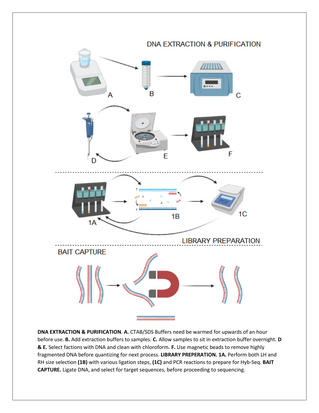
\includegraphics[width=0.9\textwidth,height=\textheight]{../graphics/assorted/molecular_metagenomic_workflow.resized.png}
\end{frame}

\begin{frame}{plant genomic reference dna - 4.4.2}
\protect\hypertarget{plant-genomic-reference-dna---4.4.2}{}
\begin{itemize}
\tightlist
\item
  38 species to sequencing
\item
  13 species duplicate
\item
  24 silica gel dried, 14 herbarium leaf tissue (RM, ID, IDS)
\end{itemize}

\begin{figure}
\centering
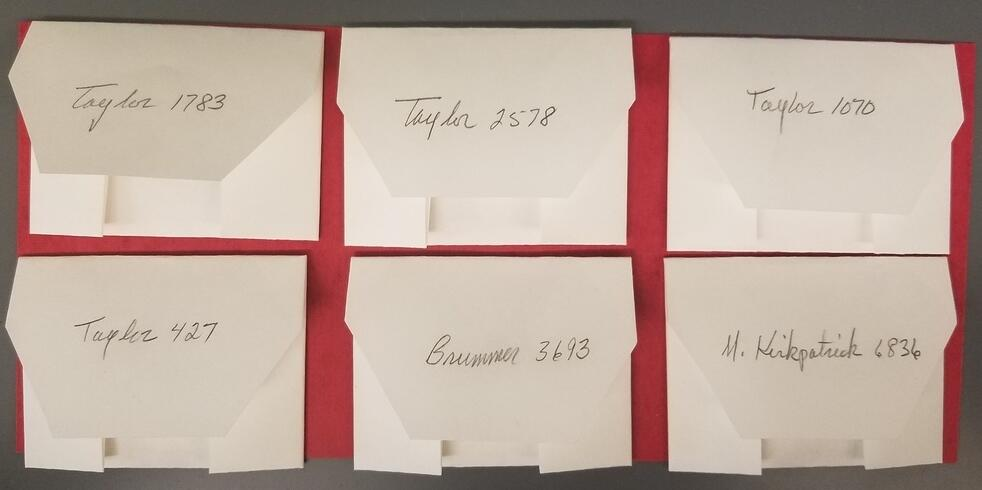
\includegraphics[width=0.65\textwidth,height=\textheight]{../graphics/pictures/Bernie_Tissue.jpg}
\caption{tissue from Rocky Mountain Herbarium}
\end{figure}
\end{frame}

\begin{frame}{pollen genomics dna - 4.4.3}
\protect\hypertarget{pollen-genomics-dna---4.4.3}{}
\begin{itemize}
\tightlist
\item
  54 Initial samples for extraction\\
\item
  44 samples underwent all steps and were analyses
\end{itemize}

\begin{figure}
\centering
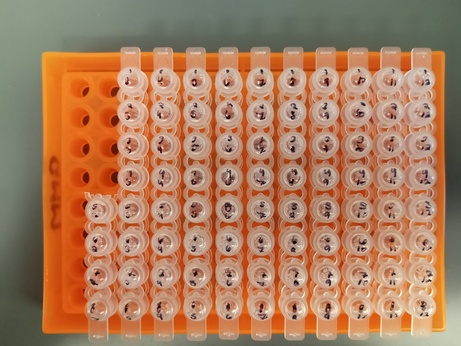
\includegraphics{../graphics/pictures/hyb-seq.resized.jpg}
\caption{hyb-seq}
\end{figure}

\note{}
\end{frame}

\begin{frame}{barcoding informatics - 4.4.4}
\protect\hypertarget{barcoding-informatics---4.4.4}{}
\begin{itemize}
\tightlist
\item
  trimmomatic, remove tags, select sequences \textgreater{} 31 bp in
  length
\item
  Kraken - qualitative identification
\item
  Bracken - quantitative identification
\item
  BLAST followup
\end{itemize}
\end{frame}

\begin{frame}{metabarcoding - 4.5}
\protect\hypertarget{metabarcoding---4.5}{}
\end{frame}

\begin{frame}{sequence database generation - 4.5.1}
\protect\hypertarget{sequence-database-generation---4.5.1}{}
\begin{itemize}
\tightlist
\item
  Kew Tree of Life \textasciitilde{} \#\#\# taxa
\item
  US \textasciitilde{} xx TAXA
\end{itemize}
\end{frame}

\begin{frame}{sequence assignment - 4.5.2}
\protect\hypertarget{sequence-assignment---4.5.2}{}
\end{frame}

\begin{frame}{semi-quantitative evidence 4.5.3}
\protect\hypertarget{semi-quantitative-evidence-4.5.3}{}
\end{frame}

\begin{frame}{5 \textbar{} results}
\protect\hypertarget{results}{}
\end{frame}

\begin{frame}{field work}
\protect\hypertarget{field-work}{}
\begin{itemize}
\tightlist
\item
  723 floral visitation observations (!)
\item
  36 unique plant species involved
\item
  64 corbiculae loads from Queens
\end{itemize}

\note{}
\end{frame}

\begin{frame}{sdm candidate species ????}
\protect\hypertarget{sdm-candidate-species}{}
\begin{itemize}
\tightlist
\item
  downloaded some 112k records
\item
  mostly trees from forestry surveys
\item
  bootstrap re-sampled to reduce effects of collection `hotspots'
\item
  non-present taxa begin nearly immediately\ldots{}
\item
  real occurrences taper off quickly
\end{itemize}

\begin{figure}
\centering
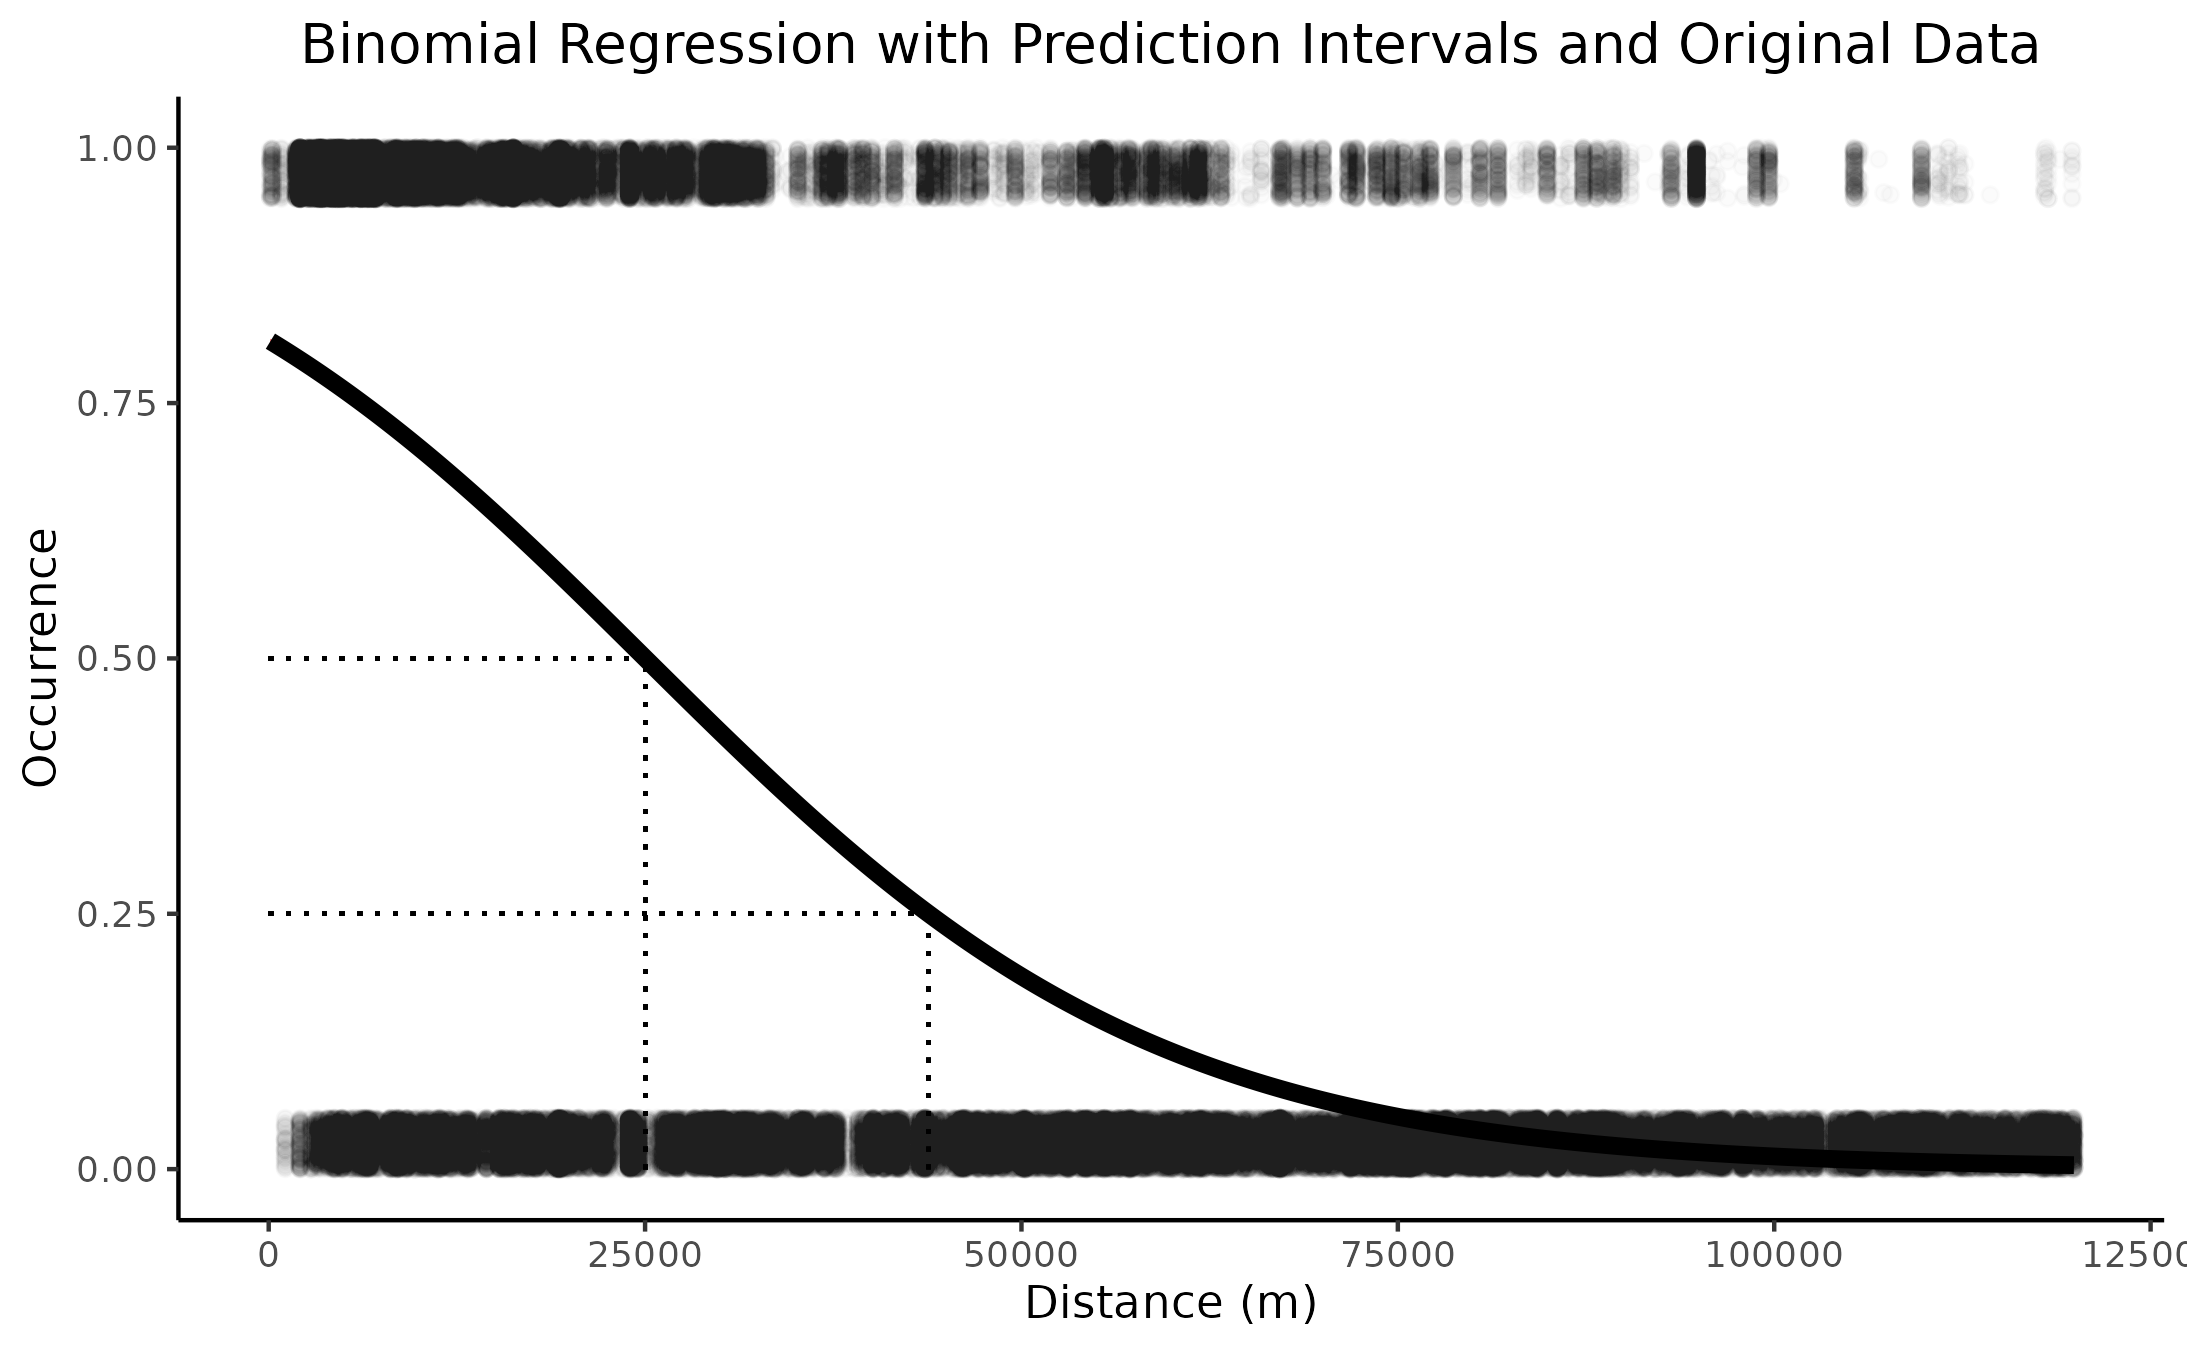
\includegraphics[width=0.9\textwidth,height=\textheight]{../graphics/plots/Occurrence_distance.png}
\caption{database}
\end{figure}
\end{frame}

\begin{frame}{sdm evaluations - computational - 5.2}
\protect\hypertarget{sdm-evaluations---computational---5.2}{}
\begin{longtable}[]{@{}lrlr@{}}
\caption{Logistic regression assessing accuracy of SDMs; witheld
data}\tabularnewline
\toprule()
Metric & Value & Metric & Value \\
\midrule()
\endfirsthead
\toprule()
Metric & Value & Metric & Value \\
\midrule()
\endhead
Accuracy (Training) & 83.75 & F-Score & 0.84 \\
Accuracy (Test) & 84.00 & AUC & 0.92 \\
Recall & 81.03 & Concordance & 0.92 \\
True Neg. Rate & 86.97 & Discordance & 0.08 \\
Precision & 88.04 & Tied & 0.00 \\
\bottomrule()
\end{longtable}

\note{Species distribution models are hypothesis which require testing.
The values in these tables arise from the practice of taking 70\% of
occurrence records and using them for training, and using the remaining
30\% of records for testing. All of these results arise from testing an
equal number of presences and absences from the final ensembled models.
From the results you can see that we focused on REMOVING more species
from the pools generated via logistic regression and distance searches
(TRUE NEGATIVE RATE), than we did on identifying presences. Overall
results were very good, and were generally highly comparable to model
performances achieved by persons focusing on modelling individual
species.}
\end{frame}

\begin{frame}{sdm evaluations - 5.3.1}
\protect\hypertarget{sdm-evaluations---5.3.1}{}
\begin{itemize}
\tightlist
\item
  able to compare to a localized vascular plant checklist

  \begin{itemize}
  \tightlist
  \item
    not everything w/ vouchers\ldots{}\\
  \item
    not everything w/ vouchers\ldots{}\\
  \end{itemize}
\item
  able to remove nearly all species from the upper (alpine) \& lower
  (sagesteppe) life zones
\end{itemize}

\begin{longtable}[]{@{}ccc@{}}
\toprule()
& ml & lm \\
\midrule()
\endhead
ensembles & 493 & 473 \\
true + & 362 & 286 \\
true - & 33 & 55 \\
false + & 64 & 41 \\
false - & 34 & 93 \\
\bottomrule()
\end{longtable}

\note{So we were able to make somewhat of a comparison to a vascular
plant checklist for the field site as a whole. The checklist is of, a
distinct quality in regards to those endeavors, and no records contain
noted vouchered accessions, no effort was made to assure the identity of
any determinations in the herbarium, and many species records are
anecdotal.

Further we did intentionally want to remove a great many of the records
from this list, which contained for example many alpine species. So it
is not a great reference, but we see that by combining the focal search
from location with SD modelling we were able to identify the presence of
many taxa.}
\end{frame}

\begin{frame}{sdm evaluations - 5.3.2}
\protect\hypertarget{sdm-evaluations---5.3.2}{}
\begin{itemize}
\tightlist
\item
  We were interested in comparison to the Valleys.
\item
  Plot Level, 117 species total (109 eligible for modelling\ldots)

  \begin{itemize}
  \tightlist
  \item
    ML: 105 (89.7\% (96.3\%))\\
  \item
    LM: 102 (87.2\% (93.5\%))
  \end{itemize}
\item
  Able to detect virtually all species recorded on plot
\end{itemize}

\note{Finally, we could compare our models in a very tangible and direct
way. We compared them to the plot level data from the plots. While these
data were not comprehensive, and hence could not be used to evaluate
absences, nor full floristic composition - we were able to predict the
presence of nearly every single species encountered on each plot. The
only taxa which we missed, which were not `restricted' from the initial
database we used to access occurrence records, were missed simply due to
taxonomic inconsistences.

As the goal of the sdm's were to predict a relevant candidate list of
species which are present in an area for developement of the database. I
believe these are very successful results.}
\end{frame}

\begin{frame}{coarse phenological modelling - 5.4.1}
\protect\hypertarget{coarse-phenological-modelling---5.4.1}{}
\begin{itemize}
\tightlist
\item
  strong agreement between first and peak flower periods with historic
  data
\item
  good agreement between last flower date
\item
  \emph{no} agreement with duration! - species do not `line up'
\end{itemize}

\begin{figure}
\centering
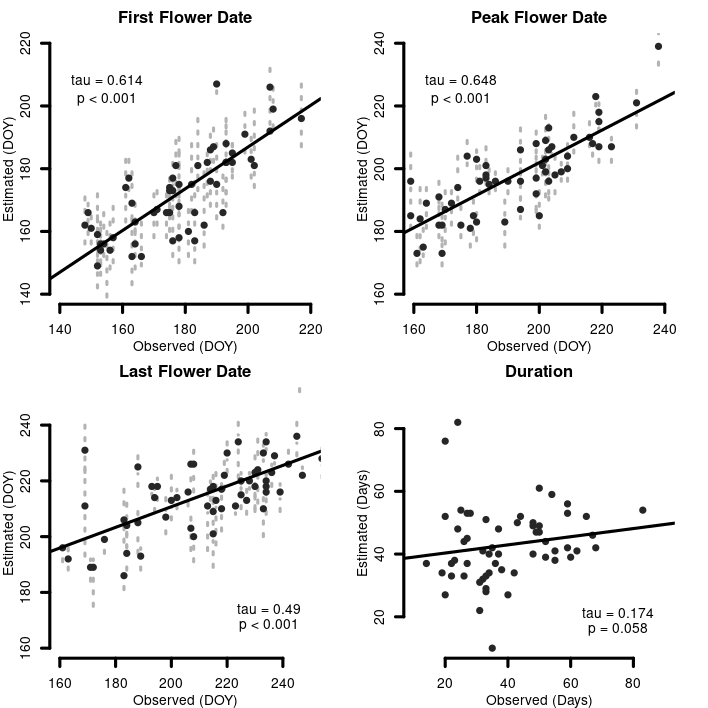
\includegraphics[width=0.92\textwidth,height=\textheight]{../graphics/plots/phenology_estimates_10_90.png}
\caption{flower dates}
\end{figure}

\note{The computational data aligned well with what has been observed on
the ground over long term periods for two calculations. There was very
good agreement between first and peak flower date, and good agreement
with last flower date. We were unable to emulate the observations of
duration. This indicates that we may not have the best data for each
individual species, but perhaps rather them as an amalgamation.}
\end{frame}

\begin{frame}{coarse phenological modelling - 5.4.2}
\protect\hypertarget{coarse-phenological-modelling---5.4.2}{}
\begin{itemize}
\tightlist
\item
  similar results with weekly data across \emph{all} field sites
  combined
\item
  tau values lower than over longer term data
\end{itemize}

\begin{figure}
\centering
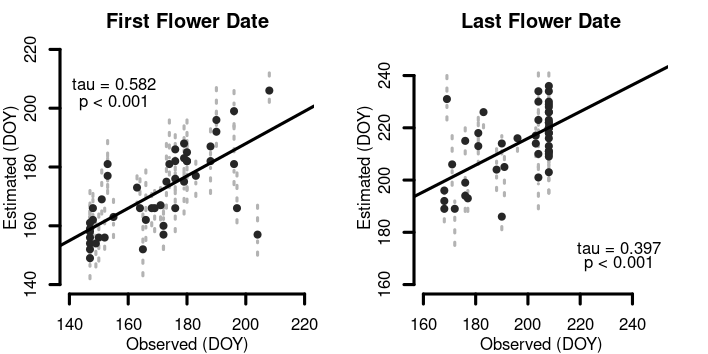
\includegraphics[width=0.5\textwidth,height=\textheight]{../graphics/plots/phenology_estimates-jeo_10_90.png}
\caption{flower dates}
\end{figure}

\note{Results were pretty much the same between the field collected data
and computationally derived data. We were not able to calculate peak
flower date due to methodological differences. We did not calculate
duration as we knew this method does not perform well in that capacity.}
\end{frame}

\begin{frame}{metabarcoding - 5.5}
\protect\hypertarget{metabarcoding---5.5}{}
\end{frame}

\begin{frame}{sequence database generation - 5.6}
\protect\hypertarget{sequence-database-generation---5.6}{}
\begin{itemize}
\tightlist
\item
  found existing data for 130 species on NCBI - SRA
\item
  novel sequence data for 25 species, varying number of loci
\item
  whole `ring' to be completed within the year
\end{itemize}

\begin{figure}
\centering
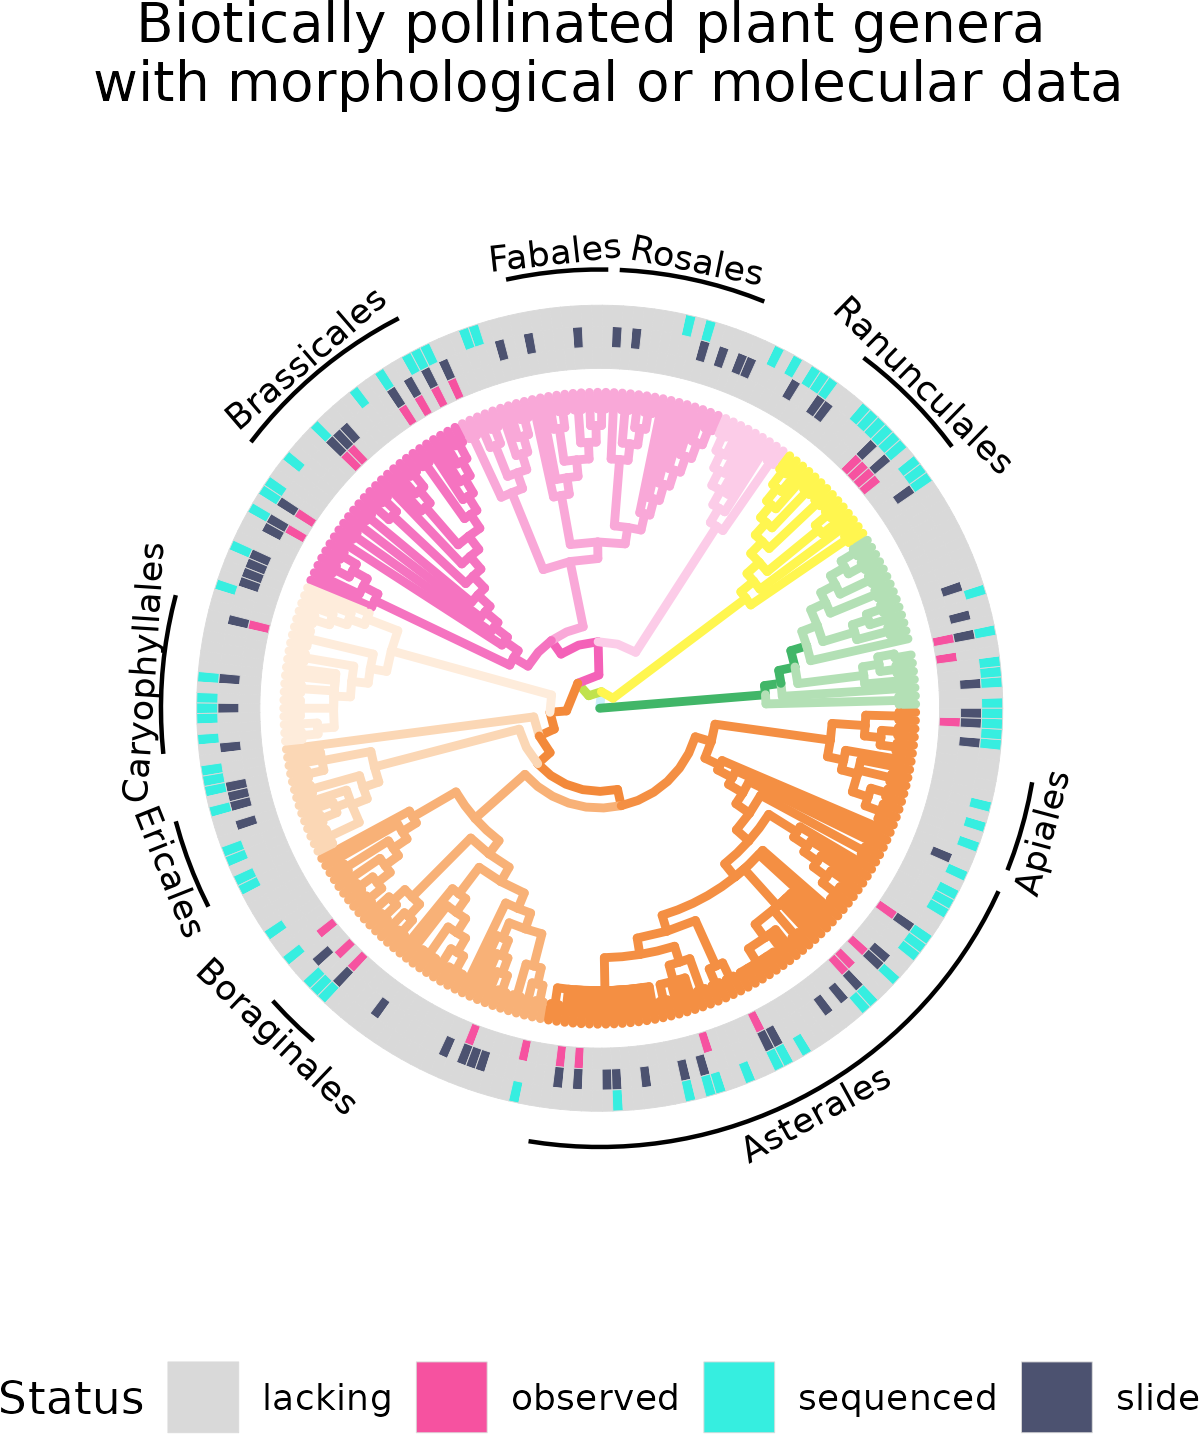
\includegraphics[width=0.9\textwidth,height=\textheight]{../graphics/plots/rmbl_draft_tree.png}
\caption{Species in Sequence DB}
\end{figure}

\note{We were not able to establish a database with nearly as much data
as we hoped to. Kew was meant to have released the full 14k species
worth of data already, but then COVID. Nonetheless, we had pretty good
coverage for our purposes. We were able to establish a database of 155
species. We expect around the time this work is published, KEW will have
released the remainder of these data.}
\end{frame}

\begin{frame}{sequence assignment - 5.7 - I}
\protect\hypertarget{sequence-assignment---5.7---i}{}
\begin{itemize}
\tightlist
\item
  trimmomatic (discard short reads)\\
\item
  Kraken (many false positives)
\item
  Bracken (many \emph{many} false positives)
\item
  Blast (fewest false positives)
\end{itemize}

\begin{figure}
\centering
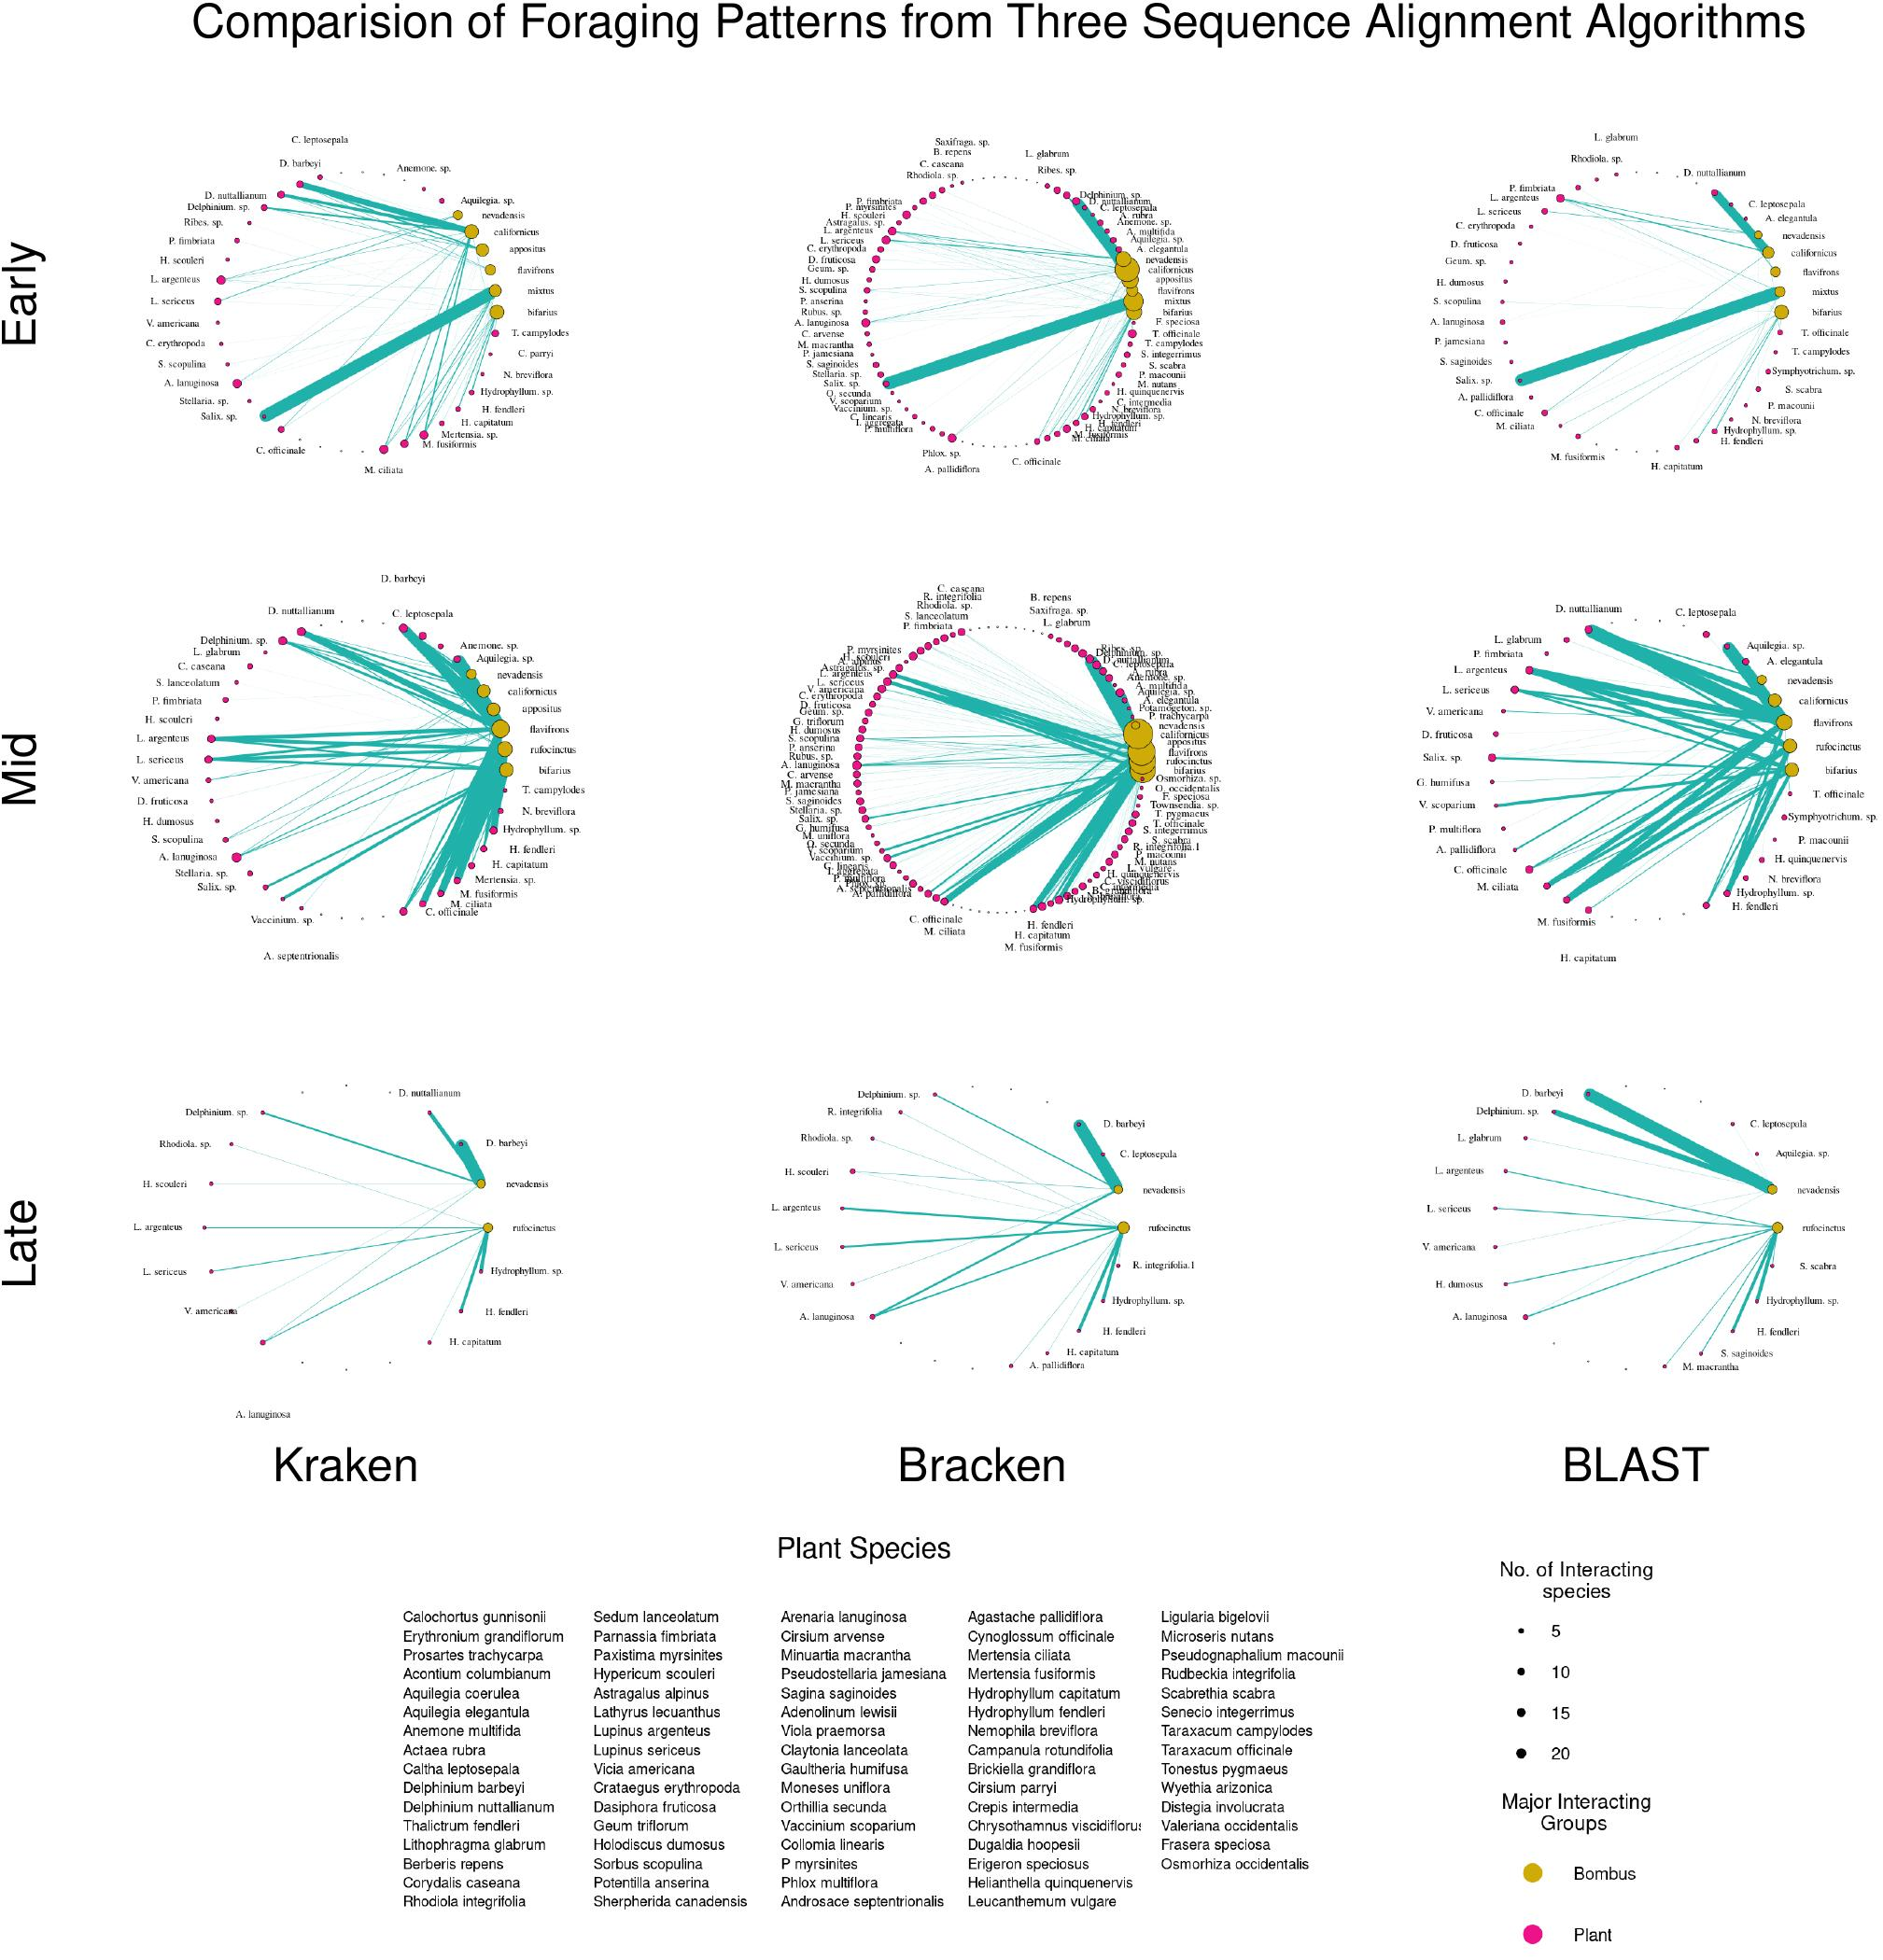
\includegraphics[width=0.93\textwidth,height=\textheight]{../graphics/plots/Molecular_nets.jpg}
\caption{Three Initial Networks}
\end{figure}

\note{We utilized trimmomatic to trim unique identifiers which are
attached to all samples for metagenomic sequencing, which have been
shown to give false positives, and to remove short reads when we were at
it. Essentially Kraken requires reads at least 30 base pairs long and
these were removed at this stage. We initially planned on using a single
algorithm for classifying our sequence reads. Kraken, kraken is a very
fast sequence alignment algorithm which has enormous popularity in the
microbiome world, and the application of metagenomics there.

Subsequent to Kraken, which will classify reads to the lowest
unambiguous taxon which it can, i.e.~it can return matches for
`Rosaceae'. Bracken `Bayesian Reestimation of Abundance with KrakEN', is
an extension of kraken which seeks to classify all reads from higher to
a terminal taxon. It also is supposedly quite good at estimating
abundances of reads in samples. We found that while Bracken would place
all results, we were very skeptical of them.

Accordingly, we decided to give BLAST, the golden standard of sequence
alignments a go. We aligned all sequences which were used by Kraken, so
essentially kraken became an intermediate filter, to BLAST. we were
considerably happier with the results from Blast being closer to what
field data told us.}
\end{frame}

\begin{frame}{sequence assignment - 5.7 - II}
\protect\hypertarget{sequence-assignment---5.7---ii}{}
\begin{table}

\caption{\label{tab:unnamed-chunk-4}Post classification of Sequences via Taxonomy and Ecology,
top 15 most abundant reads}
\centering
\begin{tabular}[t]{c|c|c|c|c}
\hline
Condition & No. Class. & Prcnt. Class. & Total Seqs & Rank\\
\hline
\cellcolor{gray!10}{A} & \cellcolor{gray!10}{143} & \cellcolor{gray!10}{21.0} & \cellcolor{gray!10}{32.0} & \cellcolor{gray!10}{Species}\\
\hline
B & 205 & 30.1 & 10.5 & Species\\
\hline
\cellcolor{gray!10}{C} & \cellcolor{gray!10}{5} & \cellcolor{gray!10}{0.7} & \cellcolor{gray!10}{0.4} & \cellcolor{gray!10}{Genus}\\
\hline
G & 29 & 4.3 & 7.8 & Species\\
\hline
\cellcolor{gray!10}{H} & \cellcolor{gray!10}{280} & \cellcolor{gray!10}{41.2} & \cellcolor{gray!10}{47.9} & \cellcolor{gray!10}{Genus}\\
\hline
None met & 18 & 2.6 & 1.4 & Multiple\\
\hline
\end{tabular}
\end{table}

\note{The number of taxa matched in any one corbiculae loads were capped
at the top 15 identifications. Using the automated sequence
reclassification schema, roughly 55\% of taxonomic records, and 50\% of
all BLAST classified sequences were moved to a species believed present
and flowering at the field station on the date the sample was collected.
Roughly 42\% of all taxonomic records, and 49\% of all blast classified
sequences were to be blunt probably wrong, and could only be placed to
the level of genus.}
\end{frame}

\begin{frame}{sequence assingment - 5.7 - III}
\protect\hypertarget{sequence-assingment---5.7---iii}{}
\begin{itemize}
\tightlist
\item
  Naive BLAST from custom databases 26\% accuracy
\item
  post-classified BLAST using temporal filters to create genera
  monogeneric in space and time 44\%
\item
  BLAST, creates \emph{many} false positives
\end{itemize}

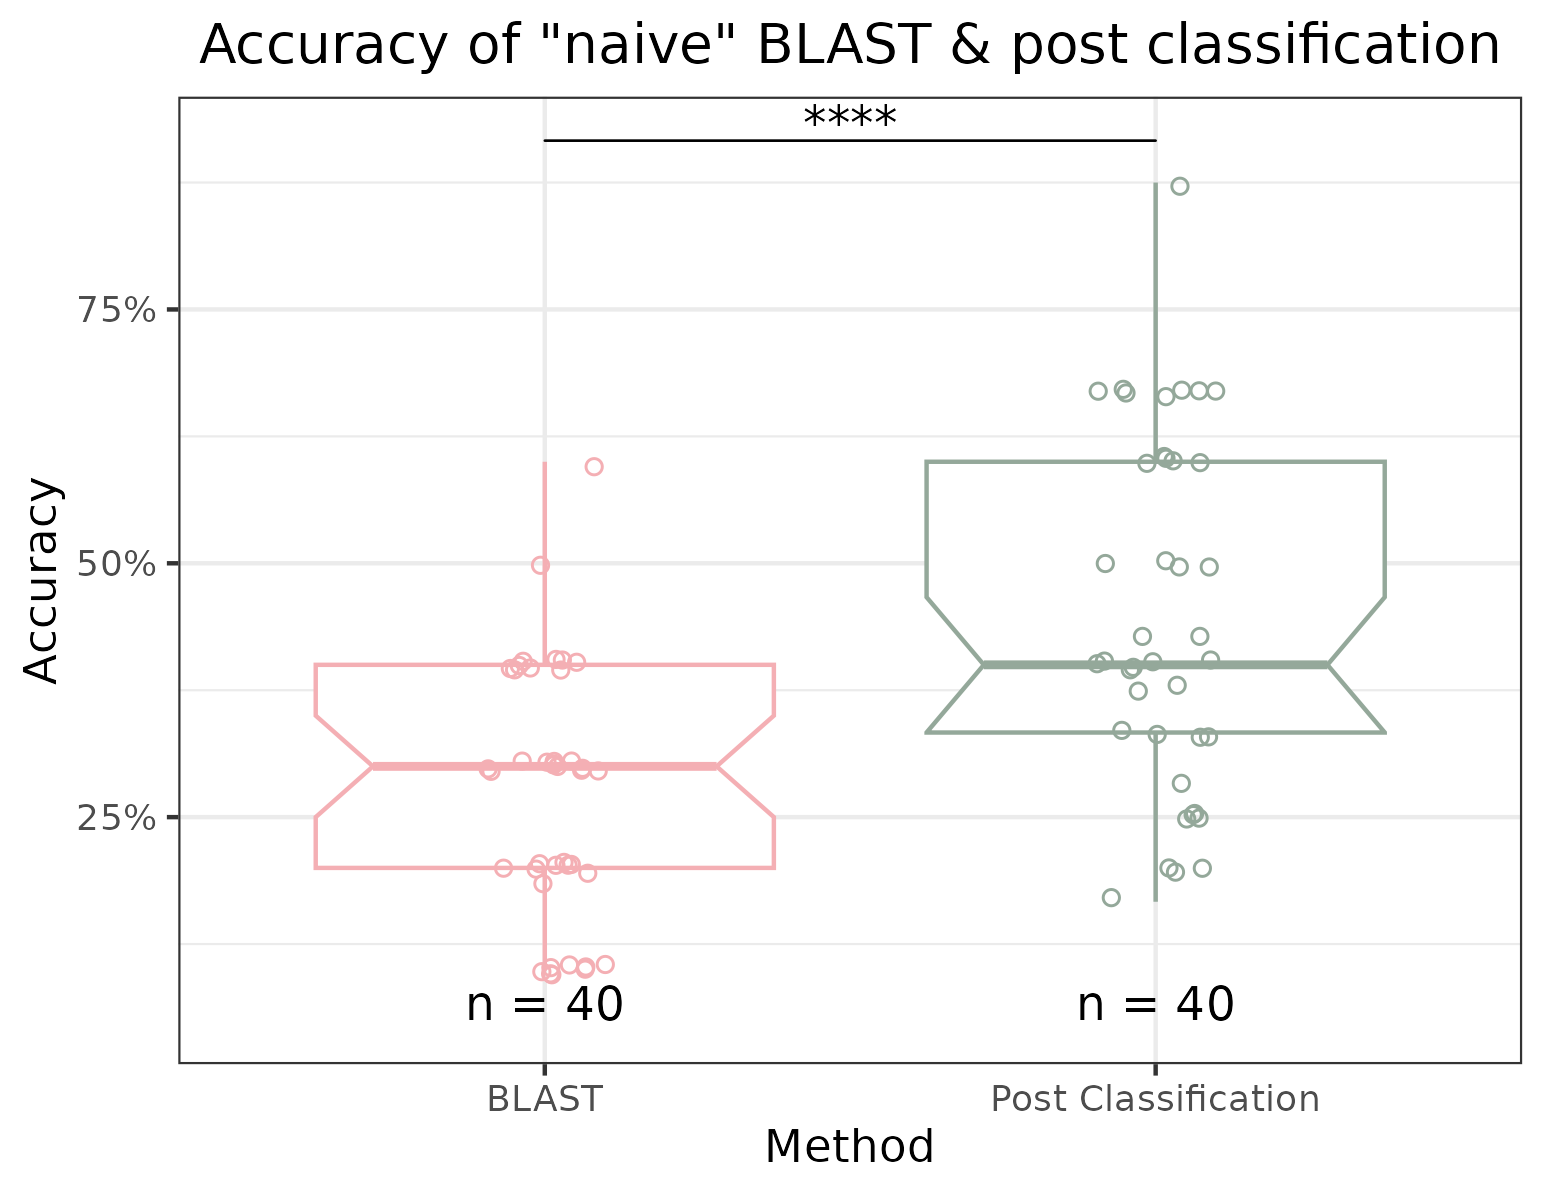
\includegraphics[width=0.95\textwidth,height=\textheight]{../graphics/plots/Accuracy_BLAST.png}
\end{frame}

\begin{frame}{sequence assingment - 5.7 - IV}
\protect\hypertarget{sequence-assingment---5.7---iv}{}
\begin{itemize}
\tightlist
\item
  conceptually similar to the automated process
\item
  utilized high resolution occurrence and phenology data
\item
  utilized morphological and molecular data
\item
  no linear operation or rule of precedence
\item
  classified all sequences to species
\end{itemize}

\note{OK so, via automatic processes, and with coarser resolution we
were missing a species identification for 50\% of our reads. But when we
have finer scale data, we can actually also classify those reads, and
reconsider the reads previously classified via the other processes.

What is very exciting about this, is this is basically the best insight
that we can get from a experts at a field station, and we can readily
compare it to the best insights which we could hope to glean from wider
expanses of land.}
\end{frame}

\begin{frame}{semi-quantitative evidence - 5.8}
\protect\hypertarget{semi-quantitative-evidence---5.8}{}
\begin{itemize}
\tightlist
\item
  \ldots{}
\item
  \emph{some} relationship exists
\item
  requires further work by someone else
\end{itemize}

\begin{figure}
\centering
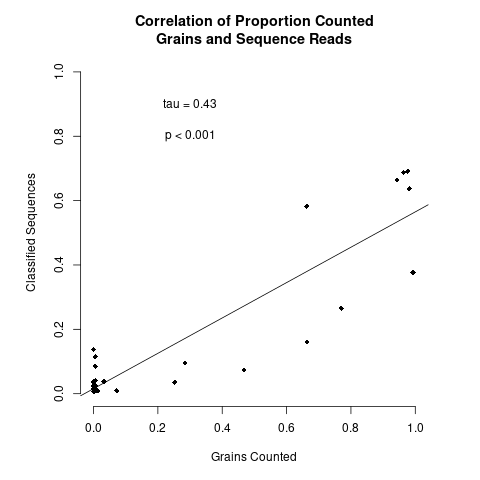
\includegraphics[width=0.92\textwidth,height=\textheight]{../graphics/plots/CorrelationCountedSequences.png}
\caption{Counted grains}
\end{figure}

\note{Alright we did use these data in the last step. SO some
relationship exists here, which seems as promising or honestly more
promising than exists for the older barcodes. We did not have much to
investigate this, but it warrants investigations.}
\end{frame}

\begin{frame}{final floral feeding structure - 5.9}
\protect\hypertarget{final-floral-feeding-structure---5.9}{}
\end{frame}

\begin{frame}{6 \textbar{} Discussion}
\protect\hypertarget{discussion}{}
\end{frame}

\begin{frame}{conservation implications - 6.1}
\protect\hypertarget{conservation-implications---6.1}{}
\begin{itemize}
\tightlist
\item
  a hidden plain text paragraph in the discussion.
\item
  collaboration with Ken Holsinger, Jedd Sondergard @ BLM Montrose
\end{itemize}

\note{I work for the Bureau of Land Management Field office immediately
adjacent to this field station. And i have been writing a lot of
reports, and I decided to sneak in a paragraph that I would be able to
cite in multiple contexts, and which would be readily interpretable to
land management professionals. So I am working with my boss and his
co-worked to refine and formulate a paragraph like this based on how to
fix these.}
\end{frame}

\begin{frame}{conservation implications - 6.1 - II}
\protect\hypertarget{conservation-implications---6.1---ii}{}
\begin{itemize}
\tightlist
\item
  historic vegetation treatment removals

  \begin{itemize}
  \tightlist
  \item
    \emph{Delphinium}, \emph{Astragalus} \& \emph{Oxytropis}\\
  \end{itemize}
\item
  altered fire cycle

  \begin{itemize}
  \tightlist
  \item
    \emph{Delphinium}, \emph{Mertensia}\\
  \end{itemize}
\item
  stream channelization / wetland removal

  \begin{itemize}
  \tightlist
  \item
    \emph{Mertensia}
  \end{itemize}
\item
  seed species, where missing
\item
  allow return of historic fire cycle, when appropriate
\item
  reintroduce beavers, or if unavailable than analogs
\end{itemize}
\end{frame}

\begin{frame}{7 \textbar{} future}
\protect\hypertarget{future}{}
\end{frame}

\begin{frame}{metabarcoding; computational approaches - 7.2}
\protect\hypertarget{metabarcoding-computational-approaches---7.2}{}
\begin{itemize}
\tightlist
\item
  qualitative:

  \begin{itemize}
  \tightlist
  \item
    search for variable loci
  \item
    flanking regions and pop gen
  \end{itemize}
\item
  quantitative:

  \begin{itemize}
  \tightlist
  \item
    read re-assignment based on phylogentic distance
  \item
    read re-assignment in bayesian framework
  \end{itemize}
\end{itemize}

\note{it seems that future uses of t}
\end{frame}

\begin{frame}{metabarcoding; new data sets? - 7.1}
\protect\hypertarget{metabarcoding-new-data-sets---7.1}{}
\begin{itemize}
\tightlist
\item
  (more) West Slope
\item
  artificial mixtures

  \begin{itemize}
  \tightlist
  \item
    leaf tissue (counted cells)

    \begin{itemize}
    \tightlist
    \item
      easier to collect
    \end{itemize}
  \item
    pollen loads (counted grains)

    \begin{itemize}
    \tightlist
    \item
      more popular
    \end{itemize}
  \end{itemize}
\item
  Gunnison Sage-Grouse scat

  \begin{itemize}
  \tightlist
  \item
    BLM habitat assessment data
  \item
    opportunistic collections
  \end{itemize}
\end{itemize}
\end{frame}

\begin{frame}{bombus; trends in perennial bunchgrasses - 7.3}
\protect\hypertarget{bombus-trends-in-perennial-bunchgrasses---7.3}{}
\begin{itemize}
\tightlist
\item
  notable declines in bunch grasses over the last 40 years
\item
  especially pronounced in montane areas
\item
  model conversion of meadows/Aspen stands to conifer forest
\item
  use existing data to model reductions in grass cover
\item
  view historic grazing renewals to monitor (loosely) reduction in grass
  diversity
\item
  forked from Ken Holsinger
\end{itemize}
\end{frame}

\begin{frame}{8 \textbar{} conclusions}
\protect\hypertarget{conclusions}{}
promising
\end{frame}

\begin{frame}{acknowledgements}
\protect\hypertarget{acknowledgements}{}
two super fantastic technicians for the field seasons I worked during
school, made my life SO easy\\
find them funding and recruit them, and then give me a finders fee.

\begin{itemize}
\tightlist
\item
  Dani Yashinowitz B.S. (Yellowstone National Park, botanist \& crew
  lead, Whitebark Pine Surveys (!!!))
\item
  Hannah Lovell B.S. (Telluride Mountain Resort, and in search of work)
\end{itemize}
\end{frame}

\begin{frame}{acknowledgments}
\protect\hypertarget{acknowledgments}{}
Employment: Yingying Xie, Josh Scholl, Sam Isham, Kelly McMillen, Kay
Hajek, Linda Vance, Cassandra Owen, Ken Holsinger

Project: Nyree Zerega, Pat Herendeen, Hilary Noble, Zoe Diaz-Martinez,
Angela McDonnell, Elena Loke, Ian Breckheimer, Ben Legler, Ernie Nelson,
Charles (Rick) Williams, D. Knoke, L. Brummer, J. Boyd, C. Davidson, I.
Gilman, M. Kirkpatrick, S. McCauley, J. Smith, K. Taylor, \& C.
Williams. David Giblin, Mare Nazaire, Sarah Burnett, Lauren Price,
T.C.H. Cole, Eliot Gardner.
\end{frame}

\end{document}
